\documentclass[a4paper,12pt,twoside]{ThesisStyle}
\usepackage[utf8]{inputenc}
\usepackage{thesis-style}
\usepackage{url}
\usepackage{booktabs}
\usepackage[table,xcdraw]{xcolor}
\usepackage{longtable}
\usepackage{lscape}
\usepackage{multirow}
\usepackage{subfig}

\begin{document}

\frontmatter

\pagenumbering{gobble}

\thispagestyle{empty}
\begin{table}[htb]
\centering
\begin{Large}
\resizebox{\textwidth}{!}{\begin{tabular}{ | l |}
 \hline
 \\

\includegraphics[scale=0.9]{imatges/logo_eps.png} \\[0.7cm]
\centerline{\textbf{Master's Degree Thesis}}\\[1cm]
\hline
\\
\textbf{Degree}: Master in Data Science\\[0.7cm]
\hline
\\
\parbox{16cm}{\textbf{Title}: The Past and Present of Predictive Models for Anomaly Detection in Smart Cities: }
\\[0.5cm]
A Systematic Review
\\[0.7cm]
\hline
\\
\textbf{Document}: Thesis\\[0.7cm]
\hline
\\
\textbf{Student}: Andrea Carolina Ramirez Moya\\[0.7cm]
\hline
\\
\textbf{Tutor}: Mateu Villaret Auselle\\
\textbf{Department}: Computer Science, Applied Mathematics and Statistics\\
\textbf{Area}: Languages and Computer Systems\\[0.7cm]
\\
\textbf{Co-Tutor}: Marc Comas Cufi\\
\textbf{Department}: Computer Science, Applied Mathematics and Statistics\\
\textbf{Area}: Statistics and Operations Research\\[0.7cm]
\hline
\\
\textbf{Call}: September 2023\\[0.7cm]
\hline

\end{tabular}}
\end{Large}
\end{table}

\newpage
\hypersetup{pageanchor=false}
\begin{titlepage}

% Upper part of the page

\includegraphics[scale=0.9]{imatges/logo_eps.png} \\[1cm]
\begin{center}
\textsc{\Large Master's Degree Thesis} \\[1cm]

% Title
\begin{spacing}{2}
\HRule \\
\textbf{\Huge The Past and Present of Predictive Models for Anomaly Detection in Smart Cities: A Systematic Review} \\
\HRule \\[0.5cm]
\end{spacing}

% Author and supervisor and other data
{
\large
\emph{Author:} \\
Andrea Carolina \textsc{Ramirez Moya} \\[1cm]
September 2023 \\[1cm]
Master in Data Science \\[1cm]
\emph{Tutors:} \\
Mateu \textsc{Villaret Auselle} \\
Marc \textsc{Comas Cufi} \\
}

\end{center}
\end{titlepage}
\hypersetup{pageanchor=true}

\titlepage

%\dominitoc


\pagenumbering{roman}

\chapter*{Abstract}
%\label{cap:resum}

Detecting anomalies in smart cities is a novel area that started being studied in the 21st century. This master's thesis aims to find the most accurate predictive models that can be explainable to scholars and industry stakeholders. With that goal in mind, a PRISMA 2020 for systematic literature reviews methodology is approached to review the papers that have been published in Emerald Insights, IEEE Xplore, Science Direct, and Web of Science with the concepts of Smart Cities, Data Science, and Predictive Models between 2000 and the first half of 2023. The findings show that the algorithms that have been studied the most are for classification, supervised machine learning. This thesis not only took into account the theoretical part, but also attempted addressing those techniques by forecasting the energy consumption in buildings in Barcelona, classifying if those outcomes were an anomaly, and finally clustering to find the consumption patterns. The deliverables are disclosed in a ObservableHQ notebook and a dashboard in Google Data Studio. 

\vspace{5mm} 
\textbf{Keywords}: Systematic Review, Predictive Models, XAI, Anomaly Detection, Smart Cities, Energy Consumption in buildings.

\vspace{10mm} 

La detecció d'anomalies en ciutats intel·ligents és una àrea nova que va començar a ser estudiada al segle XXI. Aquest treball de màster té com a objectiu trobar els models predictius més precisos que puguin ser explicables als acadèmics i a les parts interessades de la indústria. Amb aquest fi en ment, s'utilitza el PRISMA 2020 com metodologia per la revisió sistemàtica de la literatura dels treballs que han estat publicats en Emerald Insights, IEEE Xplore, Science Direct, i Web of Science amb els conceptes de Ciutats Intel·ligents, Ciència de Dades i Models Predictius entre 2000 i la primera meitat de 2023. Les troballes mostren que els algoritmes que més s'han estudiat són per a la classificació, l'aprenentatge automàtic supervisat. Aquesta tesi no només va tenir en compte la part teòrica, sinó que també va abordar aquestes tècniques mitjançant la predicció del consum d'energia en edificis de Barcelona, classificant si aquests resultats eren una anomalia, i finalment agrupant-se per trobar els patrons de consum. Els lliuraments es revelen en un quadern a ObservableHQ i un tauler de comandaments a Google Data Studio.

\vspace{5mm} 
\textbf{Paraules clau}: Revisió Sistemàtica, Models Predictius, Detecció d\'Anomalies, Ciutats Intel·ligents, Consum d'Energia en edificis, XAI.

\chapter*{Acknowledgement}

I want to express my gratitude to my supervisors Mateu Villaret Auselle and Marc Comas Cufi for their support throughout this challenging period. Their commitment to my academic development has been encouraging in the ups and downs of this journey. I value your faith in me and allowing me to gain knowledge from your guidance as I learn and grow. I genuinely thank them for their influence on my work and life.

I also want to acknowledge my professors, who should receive my sincere appreciation. Each lesson has improved my academic knowledge while shaping how I see the world. Their lectures have guided me beyond academia, so I cherish their contribution and assistance as I pursue proficiency and achievement.

I extend a heartfelt acknowledgment to my family and friends, who have been there as the base of my never-ending pursuit of knowledge. Their constant support and willingness to openly share their insights have been priceless treasures. Every conversation, brainstorming session, and word of advice has enriched my outlook and become a never-ending source of inspiration. Their presence on my journey reminds me of the significance of learning and growing together. I am grateful for their time and effort in building my awareness of the world. 

Last but not least, I would like to thank my colleagues and supervisors at Nexus Geographics. Without daring to excel in smart cities in Spain, I would not have gained the inspiration to develop this thesis. Daily learning what is going on in the industry inspired me to research this topic and helped me identify gaps in this field.


\tableofcontents

\listoffigures

\listoftables

\mainmatter

\chapter{Introduction}
\label{cap:intro}

Cities are facing a digital transformation. Part of it comes from using technology to its advantage to ensure its citizens' safety and quality of life. Governments are seeking tools to predict and alert anomalies to make informed and optimal decisions in cases of emergency to take action and address those problems. However, one limitation is that those forecasting measures must be explainable to ensure transparency and clarity in communicating with stakeholders.

This comprehensive literature review on twenty-first-century studies (2000-2023) will seek papers searched on Emerald Insights, IEEE Xplore, Science Direct, and Web of Science, in the category of Smart Cities, Data Science in the public sector, and Predictive Models. It will follow the checklist provided by the “PRISMA 2020 explanation and elaboration: updated guidance and exemplars for reporting systematic reviews”~\cite{PRISMA2020}.

No matter the size, cities need understandable models to predict their data and generate alerts on the grounds that it allows them to make informed and optimal decisions. Explainable models give them a clear and detailed account of how predictions are developing, allowing them to rely on alerts and take appropriate action to address problems detected in the public sector. Additionally, these models are easier to interpret and communicate to other stakeholders, such as citizens and department members, which can foster transparency and trust in local government.

While continuing to be fragmented and interdisciplinary, knowledge production is speeding up dramatically in the Machine Learning world. As a result, it is challenging to assess the amount of information in this field and remain on the leading edge of knowledge when selecting forecasting models. This research aims to identify a series of predictive models that are optimal in detecting and, consequently, issuing alerts in the event of finding any anomaly in the data. In this way, it will contribute significantly to improving the efficiency and effectiveness of public sector data management/governance, translating into better service and well-being for their citizens.

This research will create a solid foundation for current and future research and provide a broader and more rigorous perspective regarding possible solutions and approaches to addressing this problem. To ensure the review is accurate, a systematic review is a methodical approach for this kind of area that has been “conceptualized differently and studied by various groups of researchers within diverse disciplines”~\cite{guidelinesMNWong2019}. It will help identify, analyze, and report patterns.

All the decisions for the search strategy will be written down to enable transparency for the criteria considered when selecting and classifying the papers, the limitations encountered, and the content analysis. For this research to be thorough and robust, it will follow the four-phase guidelines “to assess the quality of a literature review”~\cite{guidelinesLRSnyder2019} that include design, conduction, analysis, and writing the review. 

Following those outcomes, with the CRISP-DM methodology, there will be an experimentation section with the electricity consumption in Barcelona to model what the authors have stated to forecast them and alert if the values are above or below the historic registers. The data will be accessed from their open data website~\cite{ElectricityBCNOD}. There’s historical data from January 2019 until March 2023. Suppose there is no access to the data types the papers are evaluating. In that case, there will be a replication section to create a dataset that complies with the aspects needed for modeling and forecasting. Once the model is trained, there will be a communication section to visualize the results found.

In Chapter~\ref{cap:prelim}, the preliminaries will explain the concepts to envision this study. In Chapter~\ref{cap:plan}, the planning and methodology will map the road to review the publications related to anomaly detection in smart cities. In Chapter~\ref{cap:estat}, the state of the art will portray the past and present of this field within the literature found. In Chapter~\ref{cap:contrib}, the experimentation will perform the anomaly detection models that have been relevant. Chapter~\ref{cap:result} will have the results from the evaluation of those approaches, and Chapter~\ref{cap:concl} will conclude this project with some discussion and future work.


\chapter{Preliminaries}
\label{cap:prelim}

This chapter presents the foundational knowledge required to comprehend this project.

\textbf{Anomaly detection.} An aspect of intrusion detection involves spotting variations from standard activity that point to intentional or accidental incidents, weaknesses, imperfections, and other problems ~\cite{omar2013machine}.

\textbf{Big Data.} Defined by its 5-v attributes: Volume, Velocity, Veracity, Variety, and Value. It refers to the immense, diverse, and complex environment for data structures (unstructured/semi-structured) that are challenging to index, sort, store, search, analyze, and visualize for use in future processes ~\cite{naeem2022trends}.

\textbf{Databases of bibliographical references.} Platforms to search bibliographic information, such as words, that describe the publication, for instance: the title, authors, abstract, and keywords ~\cite{Lund2023}. 

\textbf{Data management/governance.} The practice of authority and control over the handling of data. It seeks to maximize the value of data while reducing the cost and risk associated with its use ~\cite{abraham2019data}. 

\textbf{Data visualization.} A tool to explain discoveries to others. It helps comprehend, identify patterns, and analyze insights. Its purpose is to provide the information needed in a way that will help them perceive and think clearly with the least biases possible ~\cite{andrienko2020big}. 

\textbf{Forecasting measures.} Projections based on data with historical time stamps. It entails creating models to draw conclusions and guide strategic decision-making in the future. It is not always an accurate prediction, and forecast probabilities might vary considerably—especially when dealing with the variables that frequently vary in time series data and with external factors ~\cite{Tableau2023}.  

\textbf{K-Means.} Unsupervised machine learning algorithm that divides points in some dimensions into an established number of clusters ~\cite{hartigan1979algorithm}.

\textbf{K-Nearest Neighbor.} Supervised machine learning algorithm that is the most straightforward categorization methods that has been employed since the 90s ~\cite{laaksonen1996classification}.

\textbf{Machine learning.} It is a method through which computers run algorithms to carry out tasks while learning from data in a supervised or unsupervised way ~\cite{wazid2022uniting}.

\textbf{Open Data websites.} A platform where data is publicly accessible to anyone. It can be utilized for personal or professional reasons. It gathers transport, weather, finance, health, education, policies, and more data ~\cite{talukder2019determinants}.

\textbf{Predictive models.} A data-driven model that, given a specific input, makes a probabilistic forecast about the presence of a particular current result in the short or long term ~\cite{de2022guidelines}. 

\textbf{Smart cities.} It outlines a local entity, such as an entire city, region, or small area, that employs information technology in an integrated way with real-time analysis to promote sustainable economic growth ~\cite{Kulkarni2016}.

\textbf{Systematic review.} An assessment that compiles and summarizes information from research that answers a specific topic using specified, methodical techniques ~\cite{PRISMA2020}. 

\renewcommand{\arraystretch}{2}
\begin{longtable}{c l}
\caption{List of used acronyms and abbreviations.} \\
\parbox{2.7cm}{\textbf{Acronyms and abbreviations}} & \textbf{Definition} \\
 \\
\hline
\endfirsthead
  \parbox{2.7cm}{\textbf{Acronyms and abbreviations}} & \textbf{Definition} \\
   \\
\hline 
\endhead
\hline 
\endfoot
BSTS & Bayesian Structural Time Series \\
CatBoost & Categorical Boosting \\
COSMO & Consensus self-organized models approach \\
CRISP-DM & Cross Industry Standard Process for Data Mining\\
DBSCAN & Density-Based Spatial Clustering of Applications with Noise  \\
DTW & Dynamic Time Warping \\
GBoost & Gradient Boosted trees \\
IoT & Internet of Things\\
K-D tree & K-Dimensional tree\\
KNN & K-Nearest Neighbor \\
ML & Machine Learning \\
NB & Naive Bayes \\
LightGBM & Light Gradient Boosting \\
OBADA & Occupancy Based Anomaly Detection Algorithm \\
PARX & Poisson Autoregressions with Exogenous Covariates\\
PRISMA & \parbox{10cm}{Preferred Reporting Items for Systematic Reviews and Meta-Analyses} \\
RF & Random Forest \\
RS & Recommendation System \\
RUSBoost & Random Under Sampling Boosted trees \\
SAX & Symbolic Aggregate Approximation\\
SHAP & Shapley additive explanations \\
SVM &  Support Vector Machine \\
XAI & Explainable Artificial Intelligence \\
XGBoost & Extreme Gradient Boosting \\
\label{taula:acronyms_abbreviations}
\end{longtable}

\chapter{Planning and Design for the Methodology}
\label{cap:plan}

The methodology used in this master's thesis is divided into two distinct approaches that operate independently—one for the systematic literature review, and another for the experimentation with those results. 

Planning plays an essential role in this project to provide a clear direction, lower limitations, and ensure timely completion. Defining specific goals and objectives and laying out an approach for achieving them lays a solid basis for this project's success. Having estimated deadlines (table~\ref{taula:planning}) ensures a comprehensive layout for all the sections that must be fulfilled for a thorough project. 

\renewcommand{\arraystretch}{1.5}
\begin{table}[]
\begin{tabular}{lcc}
\multicolumn{1}{c}{\textbf{Description}} & \textbf{Estimated time} & \textbf{Actual Effort} \\
\rowcolor[HTML]{EBF4E2} 
{\color[HTML]{333333} \textbf{Project definition}} &  {\color[HTML]{333333} \textbf{3 weeks}} & {\color[HTML]{333333} \textbf{6 weeks}} \\
Research question & - & 17/04/23 - 23/05/23  \\
Supervisor's feedback & - & 01/05/23 - 08/05/23  \\
Committee acceptance & 19/05/23 & 24/05/23  \\
\rowcolor[HTML]{E1EED3} 
\textbf{Literature review} & \textbf{7 weeks} & \textbf{11 weeks} \\
\parbox{4.5cm}{Planning and design methodology} &  25/05/23 - 01/06/23 & 25/05/23 - 08/06/23 \\
\parbox{4.5cm}{Search and extraction on bibliographical databases} & 01/06/23 & 05/06/23 \\
\parbox{4cm}{Selection of papers to review} & 01/06/23 - 08/06/23 & 01/06/23 - 18/06/23   \\
Content analysis & 08/06/23 - 21/06/23 & 18/06/23 - 08/07/23  \\
\parbox{4.5cm}{Results selection for the experimentation} & 21/06/23 - 01/07/23  &  08/07/23 - 10/08/23 \\
Supervisor's feedback & 08/07/23 & 20/07/23\\
\rowcolor[HTML]{D3E6BE} 
\textbf{Experimentation} & \textbf{5 weeks} & \textbf{7 weeks} \\
Methodology design & 15/07/23 - 21/07/23 & 15/07/23 - 21/07/23 \\
Field knowledge & 21/07/23 - 28/07/23 & 21/07/23 - 04/08/23 \\
Dataset knowledge & 28/07/23 - 04/08/2023 & 04/08/23 - 20/08/23\\
\parbox{4.5cm}{Dataset preparation for modeling} & 04/08/2023 - 18/08/23 & 11/08/23 - 25/08/23\\
Dataset training & 04/08/23 - 18/08/23 & 18/08/23 - 31/08/23\\
Model evaluation & 04/08/23 - 18/08/23& 18/08/23 - 31/08/23\\
Data visualization & 04/08/23 - 18/08/23 & 25/08/23 - 31/08/23\\
\rowcolor[HTML]{CDE2B6} 
\textbf{Wrapping-up} & \textbf{1 week} & \textbf{1 week} \\
Conclusions & 21/08/23 - 28/08/23 & 01/09/23 - 05/09/23 \\
Future research & 21/08/23 - 28/08/23 & 01/09/23 - 05/09/23 \\
Abstract & 21/08/23 - 28/08/23 & 01/09/23 - 05/09/23\\
Supervisor's feedback & 01/09/23 & 06/09/23 \\
\parbox{4cm}{Draft corrections and submission} & 05/09/23 & 05/09/23 \\
\rowcolor[HTML]{C3DCA7} 
\textbf{Dissertation} & \textbf{3 weeks} & \textbf{2 weeks}\\
Designing the slides & 01/09/23 - 08/09/23 & 05/09/23 - 15/09/23\\
Presentation & 18/09/23 & 18/09/23                                         
\end{tabular}
\caption{Planning to schedule the performance for this project.}
\label{taula:planning} 
\end{table}

\section{Methodical approach for the literature review}
A literature review's main objective is to inspect and critically assess prior studies and scholarly writings on a particular subject, in this case, predictive models for anomaly detection in smart cities. This section wants to find the answers to:

\begin{itemize}
  \item Which area of a city has been studied the most, and which areas are in need of development?
  \item Which predictive models are being used on anomaly detection in smart cities? Are those models using supervised or unsupervised machine learning techniques?
  \item Which databases of bibliographical references has the most resources?
\end{itemize}

As PRISMA~\cite{PRISMA2020} states on its checklist, the first thing to do is to describe the review's criteria for inclusion and exclusion, along with how the studies are categorized for analysis. For that reason, Table~\ref{taula:SearchConcepts} was created with primary and secondary concepts relevant to this research for filtering purposes, "where in one column we write down each of the terms associated with each concept in all of its variants" ~\cite{SearchStrategy2018}. It will allow for delimiting and classifying the studies more precisely, as well as saving time and effort by not performing a comprehensive review of material that does not fulfill the criteria for this thesis.

The concepts for smart cities were taken from the six-axes that are presented in the paper \textit{"Smart Cities in Europe"}, ~\cite{allam2019big}, and ~\cite{singh2022decade},  where they also state that a city is smart when "investments in human and social capital and traditional and modern (ICT- Information and Communication Technologies) communication infrastructure fuel sustainable economic growth and a high quality of life, with a wise management of natural resources, through participatory governance"~\cite{SmartCitiesEurope2011}. 

In order to enhance decision-making and deliver better services to people, city data gathered from many sources, including sensors, internet-connected devices, and other external sources, is extracted for relevant insights and hidden connections ~\cite{SmartCitiesDataScience2022}. For that reason, and also adding the concepts learned throughout the master is essential for the part of the system environment that houses the large amount of data that a city captures every single day. 

Finally, for the third key concept of this project, which is predictive models for anomaly detection, the review will need to center on classifying or clustering data using explainable approaches that enhance transparency when interpreting and communicating them to other stakeholders. 

\renewcommand{\arraystretch}{1.5}
\begin{table}[htb]
\centering
\begin{tabular}{ | l | l | l | }
 \hline
  \textbf{Smart Cities} & \textbf{Data Science} & \textbf{Anomaly detection} \\
\hline
 Economy & Sensors & Supervised Machine Learning \\
 Mobility  &  Internet of Things & Unsupervised Machine Learning \\
 Environment  & Data Models & Time Series\\
 People & Data Architecture & \\
 Living & Data Engineering & \\
 Governance &  & \\
  \hline
  \end{tabular}
\caption{Concepts to review.}
\label{taula:SearchConcepts} 
\end{table}

The papers will be retrieved depending on their published date, which fits the limit between January 1st, 2000, until June 1st, 2023 (this century), and the concept to review from the primary sources that are at the bibliographical references databases: \textit{Emerald Insights}, \textit{IEEE Xplore}, \textit{Science Direct} and \textit{Web of Science}. One reason to select these databases is that they have the largest open-access collection, making scientific knowledge and research available to everyone, free from limitations like cost or membership, making reachable information for researchers and the general public.

These databases were selected based on their expertise in a broad range of academic and scientific fields. It was important to extract papers from \textit{IEEE Xplore} for this project since it focuses on engineering and computer science. However, finding only two papers qualified for extraction was shocking. In virtue of that limitation, the conference papers were also selected for review. 

\begin{table}[htb]
\centering
\begin{tabular}{  c  l   }
 \hline
  \textbf{Search} & \textbf{Search strategy} \\
\hline
 \#1 & \parbox{11.5cm}{Smart Cities AND Data Science AND Predictive Models}  \\
 \#2 & \parbox{11.5cm}{Data Science AND Anomaly detection}   \\
 \#3 & \parbox{11.5cm}{Smart Cities AND Anomaly detection}   \\
 \#4 & \parbox{11.5cm}{Smart Cities AND Data Science AND Anomaly detection}  \\
  \\
 \#5 & \parbox{11.5cm}{\#4 AND (Economy OR Mobility OR Environment OR People  OR  Living OR Governance OR Sensors OR Internet of Things OR Smart Data Models OR Data Acquisition OR Data Architecture OR Data Engineering OR Data visualization OR Supervised Machine Learning OR Unsupervised Machine Learning)}  \\
  \\
 \#6 & \parbox{11cm}{\#5 AND NOT Blockchain [Title/Keywords] AND NOT Deep Learning [Title/Keywords] AND NOT Neural Networks AND NOT Federated Learning AND NOT Reinforcement Learning AND NOT Cloud/Fog Computing [Title/Keywords]}  \\
 \\
  \hline
  \end{tabular}
\caption{Search strategy.}
\label{taula:SearchStrategy} 
\end{table}

\begin{figure}[htb]
\centering
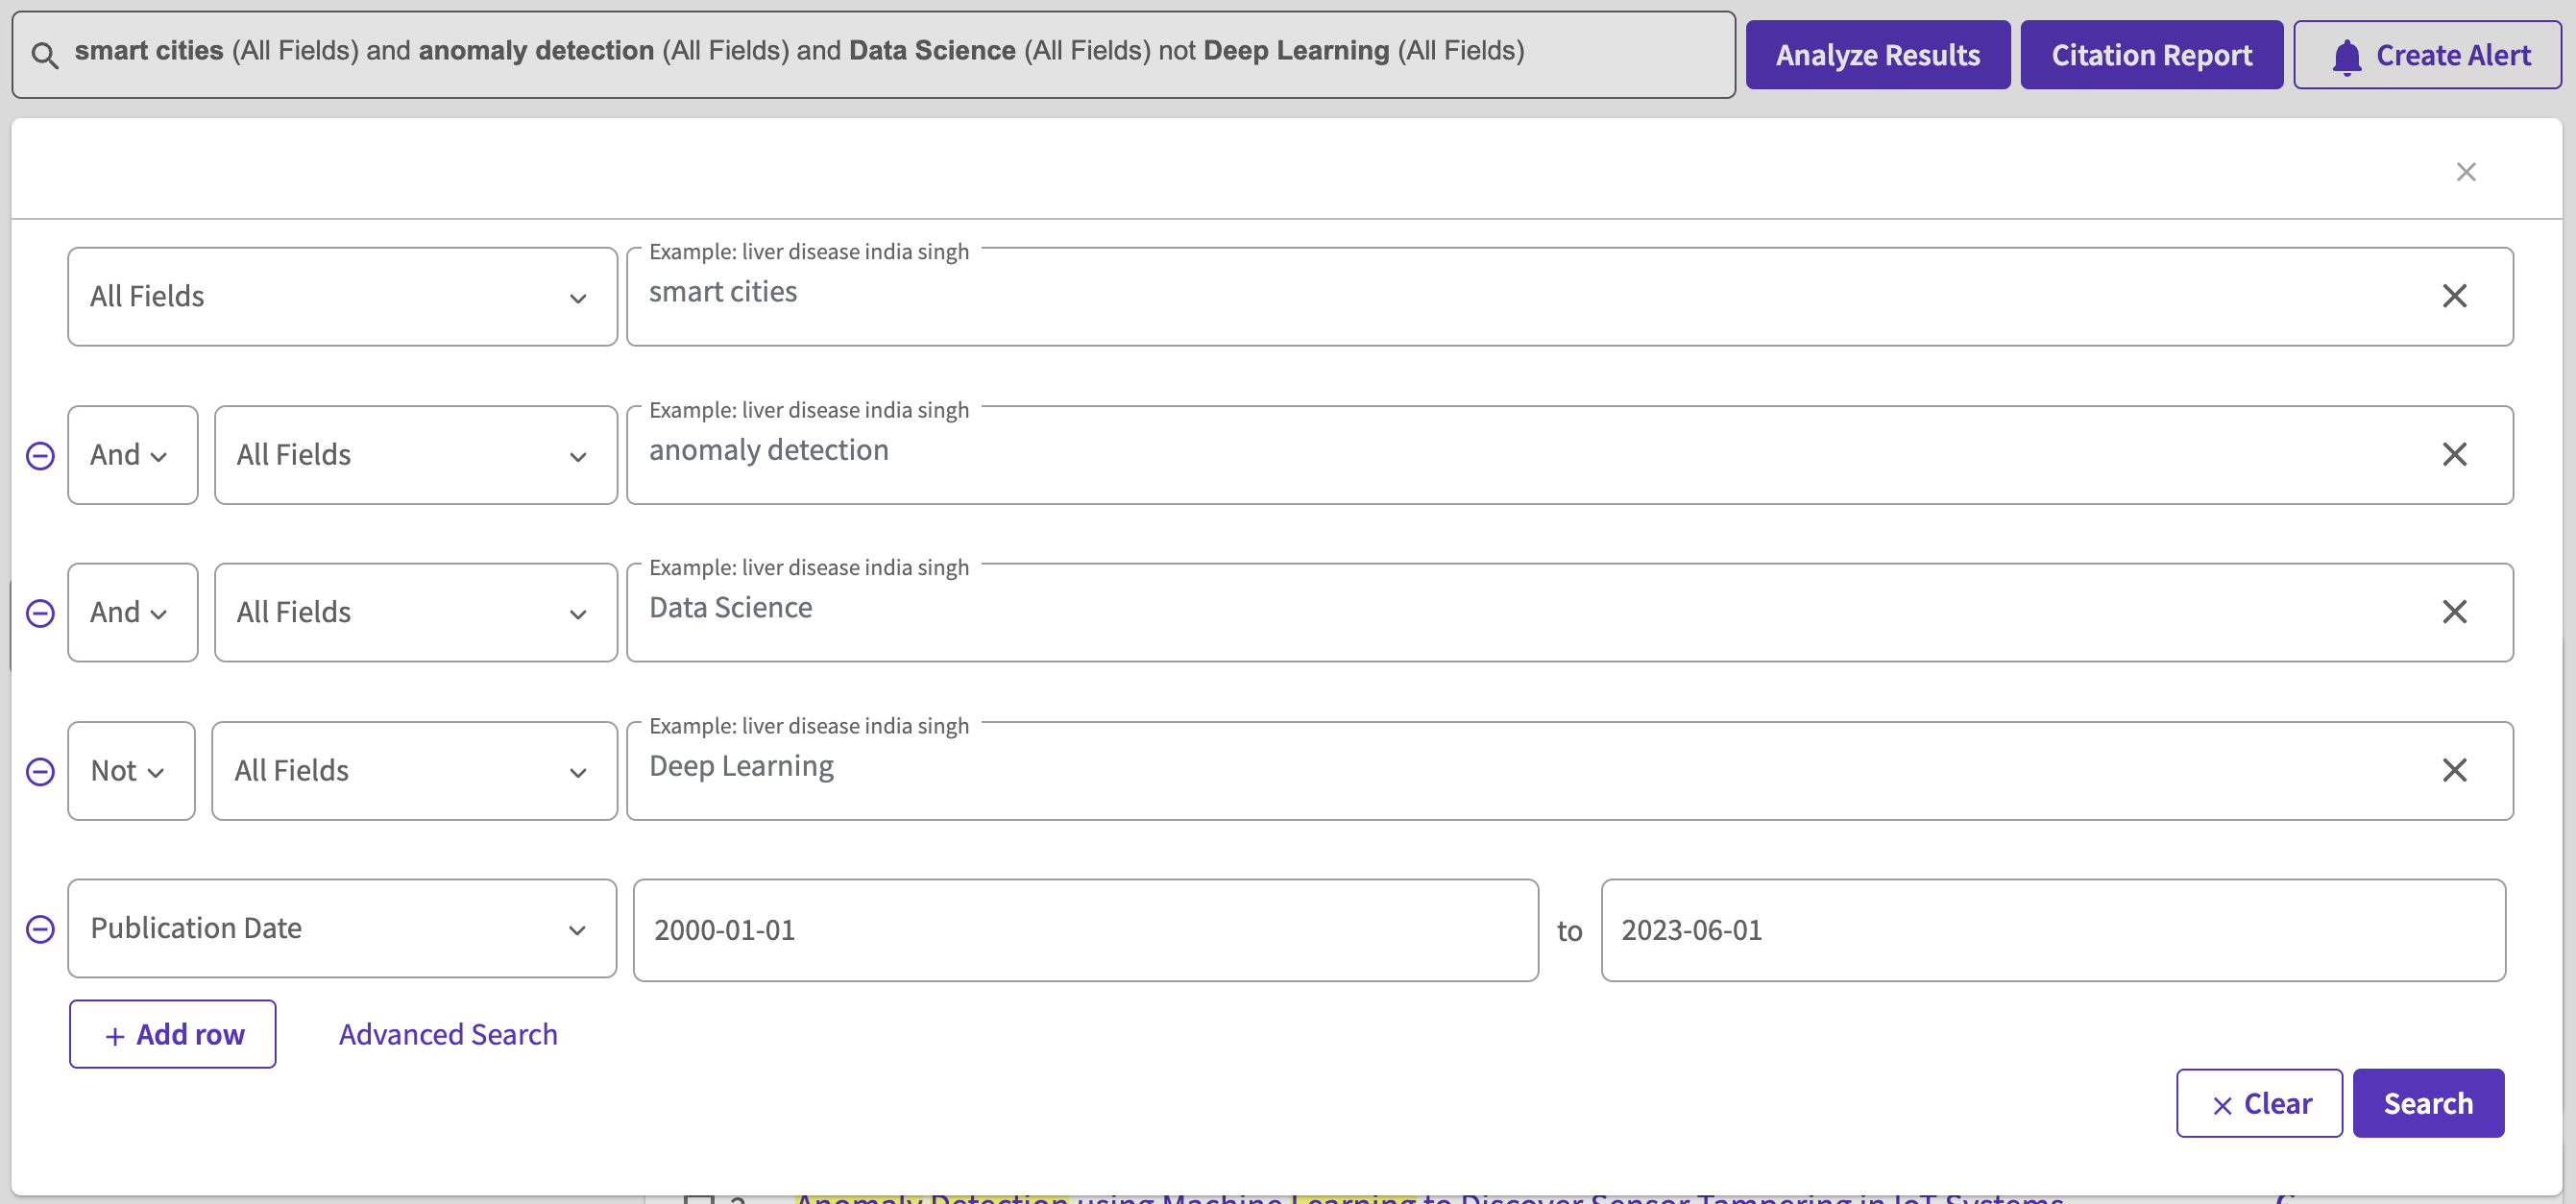
\includegraphics[width=13 cm]{imatges/search_concepts.png}
\caption{\label{fig:search_concepts} Advanced settings to extract the papers on the \textit{Web of Science} using part of the strategy \#5.}
\end{figure}

With the Boolean operator AND, papers can be identified  that include the primary concepts from the search strategy  ~\cite{SearchStrategy2018} ~\cite{SystematicLiteratureReviewsEngineering2014} (table~\ref{taula:SearchStrategy} and an example of retrieval on figure~\ref{fig:search_concepts}). The strategy \#4: Smart cities AND Data Science AND Anomaly detection was used because by filtering the other way around, 1,000 papers would be needed to be reviewed. On that iteration of searching on each bibliographical database, 377 papers were downloaded (table~\ref{taula:FoundPapers}). However, several studies are not relevant to this review since they are related to Blockchain, Cloud, Edge, and Fog Computing, Deep Learning, Reinforcement Learning, Adversarial Learning, and Federated Learning, which are out of the scope of explainable predictive modeling. Therefore, this is the moment to benefit from selecting secondary concepts and filtering those papers that contain at least one relevant keyword or term in their title. That led to 277 papers to review (strategy \#5 and strategy \#6).

"At the end of our search, we need to assess the results obtained, both in exhaustiveness (provision of relevant documents which a strategy has been capable of finding), and precision (number of relevant records retrieved compared with the total number of retrieved records) and relevance (which will be useful) to respond to our question" ~\cite{SearchStrategy2018}. Some papers could be listed in different databases, so it is critical to identify them to measure the studies' precision and relevance. For that reason, those papers were screened by keywords and abstract to ensure the studies were within this project's scope. That left us with 45 papers to review comprehensively.

\renewcommand{\arraystretch}{2}
\begin{table}[htb]
\centering
\begin{tabular}{ | r | c | c | c | c | c | }
 \hline
  \textbf{Database} & \parbox{1.5cm}{\textbf{Emerald Insights}} & \parbox{1.5cm}{\textbf{IEEE Xplore}} & \parbox{1.5cm}{\textbf{Science Direct}} & \parbox{1.5cm}{\textbf{Web of Science}} & \textbf{Total} \\
\hline
 \parbox{3.7cm}{\textit{Records retrieved on strategy \#1}} & 91 & 52 & 982 & 47 & \textbf{1.172} \\
 \parbox{3.7cm}{\textit{Records retrieved on strategy \#2}} & 53 & 621 & 830 & 510 & \textbf{2.014} \\
 \parbox{3.7cm}{\textit{Records retrieved on strategy \#3}} & 13 & 22 & 812 & 134 & \textbf{981} \\
 \parbox{3.7cm}{\textit{Records retrieved on strategy \#4}} & 10 & 58 & 282 & 24 & \textbf{377} \\
 \parbox{3.7cm}{\textit{Records retrieved on strategy \#5}} & 10 & 50 & 200 & 21 & \textbf{281} \\
 \parbox{3.7cm}{\textit{Records retrieved on strategy \#6}} & 6 & 50 & 200 & 21 & \textbf{277} \\
 \parbox{3.7cm}{\textit{Screened by keywords}} & 6 & 50 & 67 & 21 & \textbf{144} \\
 \parbox{3.7cm}{\textit{Screened by abstract}} & 1 & 6 & 29 & 9 & \textbf{45} \\
  \hline
  \end{tabular}
\caption{Papers retrieved.}
\label{taula:FoundPapers} 
\end{table}

\begin{figure}[htb]
\centering
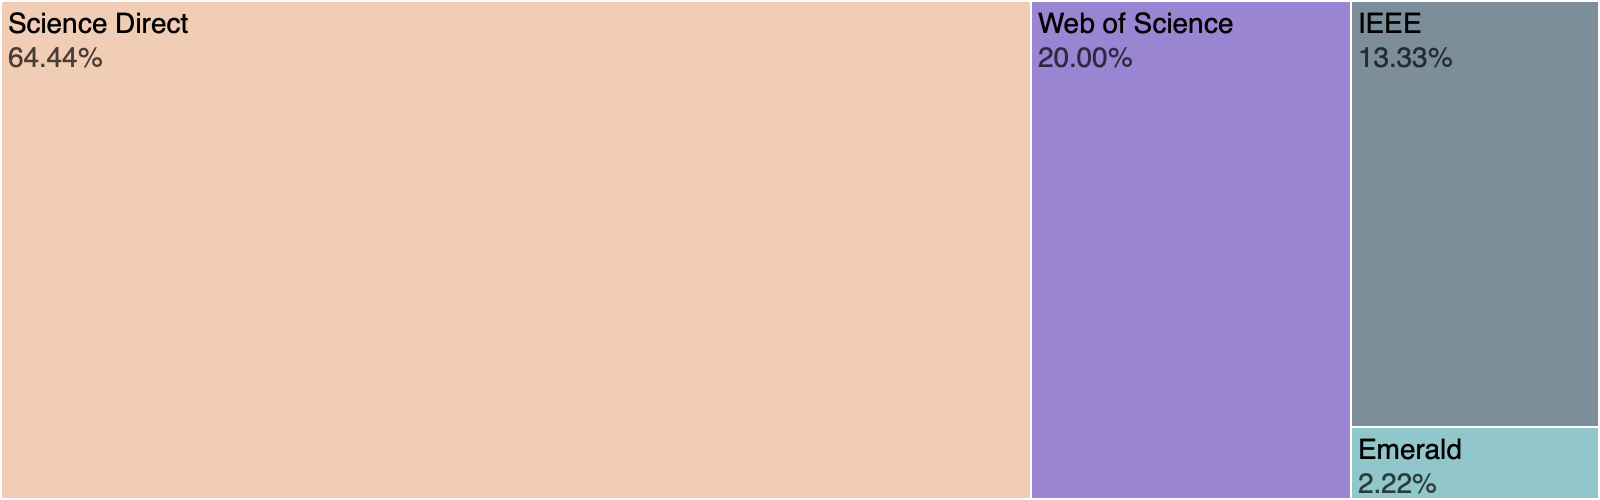
\includegraphics[width=13 cm]{imatges/referenceDB.png}
\caption{\label{fig:referenceDB} Share of reference databases reviewed.}
\end{figure}

As seen in Table~\ref{taula:FoundPapers} and Figure ~\ref{fig:referenceDB}, the reference database that had the most papers to review was Science Direct (64\%), followed by Web of Science (20\%), IEEE (13\%), and last Emerald (2\%). 

To perform this systematic review, the four stages of content analysis proposed by ~\cite{gaur2018systematic} were followed. Hence the explanation on collecting the papers (table~\ref{taula:SearchStrategy}), and  describing the concepts to review (table~\ref{taula:SearchConcepts}). Now, for the analysis, and interpretation of coded content a \textit{Google Form} (\url{https://shorturl.at/akluK}) was created. This tool works as a replicable method based on explicit criteria for downsizing large amounts of text into reduced content categories of the different publications. Using this tool it is more manageable to count the frequency of the keywords and concepts with a manifest focus in the scope of this study. It also allows a qualitative approach by "categorization, summarization, and interpretation of textual data without using statistical interpretation"~\cite{stemler2000overview} with a latent focus.



\chapter{State of the Art - The past and present}
\label{cap:estat}

The detection of "a thing, situation, etc. that is different from what is normal or expected" ~\cite{anomalyOxford} has been performed since the beginning of time. The first time it was mentioned along with ML was in 1942 by the Scientific Research Society of North America, Society of the Sigma Xi. They studied the learning behaviors of their students and created an anomaly detection system that is flexible enough to accept "normal" changes, specified by the researchers ~\cite{Scientist1942}.

Decades later, there are records from the aeronautical industry ~\cite{Nuclear1958} and ~\cite{Aerospace1966}, where they developed computer software to approach the detection of anomalies on their several aircraft, and their air force and nuclear projects.

By 1983, there was the first publication on ML and anomaly detection. It covers inductive learning systems, learning by analogy, experimentation, experience, observation, and instruction ~\cite{anderson1983machine}. From that time forward, there is a new knowledge revolution in science.

It was not until 1995 that the \textit{Mathematical and Computer Modelling} journal published the first research on intelligent transportation systems. ~\cite{AMIN19951} and ~\cite{GARCIAORTIZ199511} explore the complexity of traffic on roads and highways and breakthroughs in computing techniques and computer systems while performing collaborative research between academia, industry, and government. 

Ever since the 80s, there has been literature regarding smart cities, where city councils adopt and launch geographic information systems on the internet with data ready to be used. However, by the end of the 20th century, several authors believed that using ML for anomaly detection was a highly neglected subject and that their research "will serve to temper the development and deployment of these Intelligent transportation programs" ~\cite{GARCIAORTIZ199511}. 

\begin{figure}[htb]
\centering
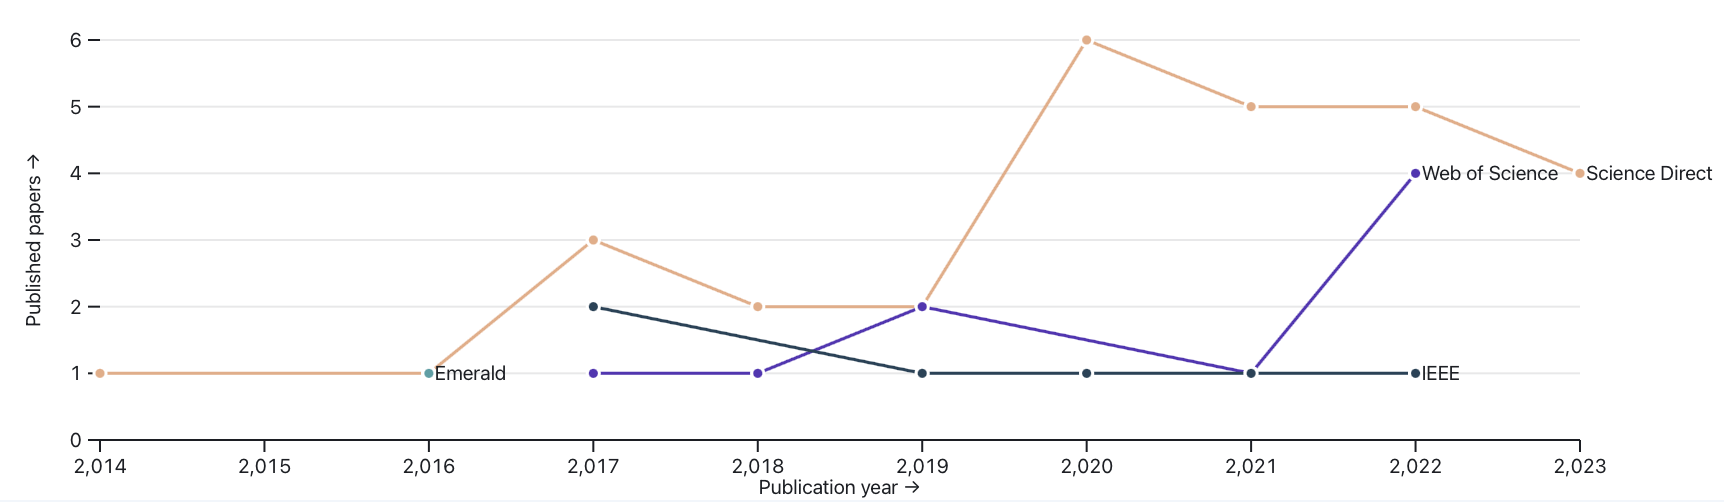
\includegraphics[width=13 cm]{imatges/publicationDB.png}
\caption{\label{fig:publicationDB} Published papers per reference databases reviewed.}
\end{figure}

It was not until 2014 in Bahrain that the first open access paper published by \textit{Science Direct} that studies anomalies in cyber security on the \textit{Journal Procedia Computer Science} (figure ~\ref{fig:publicationDB} and table~\ref{taula:PapersReviewed}). They performed a multi-criterion fuzzy classification method with greedy attribute selection for anomaly-based intrusion detection. This approach enables it to choose an ideal subset of features most relevant for identifying intrusive events, reducing the dimension of the data set, and improving computing efficiency. "The simplicity of the constructed model allows it to be replicated at various network components in emerging open system infrastructures" ~\cite{el2014multicriterion}.

In 2016, the Defense Advanced Research Projects Agency introduced the topic of XAI "to create a suite of machine learning techniques that: produce more explainable models, while maintaining a high level of learning performance (prediction accuracy); and enable human users to understand, appropriately trust, and effectively manage the emerging generation of artificially intelligent partners." ~\cite{DAR2016}. 

There is an inevitable conflict between explainability and a model learning performance. Despite that, their project discovered evidence that comprehension may boost accuracy when testing it. Their aim was admirable; however, as a system, it faced the issue that "different user types require different types of explanations. This is no different from what we face interacting with other humans" ~\cite{gunning2021darpa}.

Even though it started as a tool, it established the ground to perform explainable ML models. In the second decade of the 21st century, it was used for deep learning approaches in healthcare (~\cite{LAMY201942}, ~\cite{SABOL2020103523}, ~\cite{KAVYA2021102681}). 

In the case of anomaly detection in smart cities, the first and only time that this term was utilized was in 2022 by researchers in South Korea who experimented on electrical load forecasting of buildings where they "employed the tree SHAP method to improve the explainability of the DT-based ensemble models by computing the contribution of each input variable to the prediction" ~\cite{moon2022toward}. They also found that the LightGB model trained with external and internal parameters outperformed the other forecasting models in terms of prediction performance.

\begin{figure}[htb]
\centering

\includegraphics[width=13 cm]{imatges/keywordsDB.png}
\caption{\label{fig:keywordsDB} Keywords related to the papers reviewed.}
\end{figure}

That said, it is time to dig deeper into the scope at hand: anomaly detection in smart cities. After following the methodology proposed, 45 papers were reviewed. They were published on the four reference databases in the past decade, from 2014 until mid-2023 (figure~\ref{fig:publicationDB}). 

The peak of publishing so far has been in 2022, where \textit{Science Direct} and \textit{Web of Science} hold the most records available of open access papers. The keywords that repeated the most were \textit{Machine Learning}, \textit{Internet of Things}, \textit{Classification}, and \textit{Clustering} (figure~\ref{fig:keywordsDB}).

This review found that the area that has been researched the most is \textit{Transportation}, followed by \textit{CyberSecurity} and \textit{Energy}. This scrutiny
includes studies in 8 areas of study that also include: \textit{Education}, \textit{Environment}, \textit{Health}, \textit{People}, and \textit{Structures}.

In table~\ref{taula:PapersReviewed}, there is a classification per bibliographical reference database and the paper's area of study. Following that the chapter will be divided into the sections used as key concepts:  Section~\ref{subcap:smartcities} Smart Cities, Section~\ref{subcap:datascience} Data Science, and Section~\ref{subcap:predictivemodels} Predictive Models for anomaly detection.

\renewcommand{\arraystretch}{1.5}
\begin{longtable}{  l c l  }
\caption{Papers reviewed.}  \\
\label{taula:PapersReviewed}  \\
\hline
  \textbf{Area of study} & \parbox{3cm}{\textbf{Bibliographical Reference}} & \textbf{Papers} \\
\hline 
\endfirsthead
 \hline
  \textbf{Area of study} & \parbox{3cm}{\textbf{Bibliographical Reference}} & \textbf{Papers} \\
\hline 
\endhead
\hline
\endfoot
\multirow{2}{*}{CyberSecurity} & \textit{Science Direct} & \parbox{7cm}{~\cite{el2014multicriterion}, ~\cite{al2018semi}, ~\cite{mohamudally2018building}, ~\cite{saranya2020performance}, ~\cite{bangui2021hybrid}, ~\cite{abd2022analyze}, ~\cite{saheed2022machine}, ~\cite{bukhari2023anomaly}, ~\cite{yadav2023augmentation}} \\
 \cline{2-3} 
 & \textit{Web of Science} &  ~\cite{protic2022cybersecurity} \\
\hline 
\multirow{2}{*}{Energy}  & \textit{Emerald} &  ~\cite{gerrish2017analysis} \\
\cline{2-3}  
 & \textit{IEEE} &  ~\cite{Carbone2017heating} \\
\cline{2-3} 
 \multirow{1}{*}{Energy} & \textit{Science Direct} & \parbox{7cm}{~\cite{cerquitelli2017predicting}, ~\cite{fonseca2017unsupervised}, ~\cite{liu2018scalable}, ~\cite{du2019clustering}, ~\cite{ali2020data}, ~\cite{himeur2020data}, ~\cite{leiria2021using}, ~\cite{moon2022toward}, ~\cite{alsalemi2023modular}} \\
\hline 
\multirow{2}{*}{Environment}  &  \textit{Science Direct} &  ~\cite{vijai2016design} \\
\cline{2-3} 
 & \textit{Web of Science} &  ~\cite{hangan2022advanced} \\
\hline 
\multirow{1}{*}{Health}  & \textit{Web of Science} &  ~\cite{abu2022automated} \\
\hline
\multirow{2}{*}{People} & \multirow{1}{*}{\textit{IEEE}} & ~\cite{Zhu2020cellular}  \\ 
\cline{2-3} 
 &\multirow{1}{*}{\textit{Science Direct}}  & ~\cite{embarak2021new} \\
\hline
\multirow{1}{*}{Structures}  & \textit{IEEE} &  ~\cite{Zinno2022bridges} \\
\hline
\multirow{6}{*}{Transportation} & \textit{IEEE} & \parbox{7cm}{~\cite{Zhao2017passenger}, ~\cite{Wang2017Taxis}, ~\cite{Bawaneh2019traffic}, ~\cite{Xu2019outlier}, ~\cite{Nugraha2021rail} } \\
 \cline{2-3} 
 & \textit{Science Direct} & \parbox{7cm}{~\cite{masino2017learning}, ~\cite{killeen2019iot}, ~\cite{belhadi2020space}, ~\cite{mondal2020road}, ~\cite{gomari2021cluster}, ~\cite{kyriakou2021vehicles}, ~\cite{Wang2021CAN}, ~\cite{bachechi2022big}, ~\cite{sara2020predict}, ~\cite{karanfilovska2022analysis}, ~\cite{vidovic2022methodology}, ~\cite{wu2023gtfs} } \\
  \cline{2-3} 
 & \textit{Web of Science} &  ~\cite{zantalis2019review} \\
\end{longtable} 

\section{Smart cities}
\label{subcap:smartcities}

Several scientific methodologies, ML techniques, procedures, and systems are commonly used in data science to research and analyze real-world events utilizing historical data, that way "extracting useful knowledge or actionable insights from city data and building a corresponding data-driven model is the key to making a city system automated and intelligent" ~\cite{SmartCitiesDataScience2022}. 

For this section of the review, the latent categories from the concepts will be presented, and how they have developed in this century.

\subsection{Economy}

Most of the publications that have referred to the economy of a smart city are published by the Journal \textit{Procedia Computer Science} that is on \textit{Science Direct} bibliographical reference database (table~\ref{taula:PEconomy}). 

\renewcommand{\arraystretch}{1.5}
\begin{longtable}{  l  l  l }
\caption{Papers related to the economy in smart cities.}  \\
\label{taula:PEconomy}  \\
\hline
  \textbf{Area of study} & \textbf{Journal} & \textbf{Paper} \\
\hline 
\endfirsthead
 \hline
  \textbf{Area of study} & \textbf{Journal} & \textbf{Paper} \\
\hline 
\endhead
\hline
\endfoot
\multirow{1}{*}{Energy} & \textit{Emerald Publishing Limited} &  ~\cite{gerrish2017analysis}  \\
 \hline 
 \multirow{1}{*}{Environment} & \textit{Procedia Computer Science} &  ~\cite{mohamudally2018building}  \\
\hline 
\multirow{1}{*}{People} &  \textit{Procedia Computer Science} &  ~\cite{embarak2021new} \\
\hline 
\multirow{1}{*}{Transportation} &\parbox{5cm}{\textit{Engineering Applications of Artificial Intelligence}} &  ~\cite{belhadi2020space}  \\
\end{longtable}

The first published paper is related to building performance by researchers from Loughborough University, UK, and the professional services firm BuroHappold Engineering. They found "patterns in thermal response across monitored rooms in a single building, to clearly show where rooms are under-performing in terms of their ability to retain heat during unconditioned hours"~\cite{gerrish2017analysis}. That affects the energy payment bill, especially in an energy crisis scenario when there is demand and costs out of budget.

The following year, at the 15th International Conference on Mobile Systems and Pervasive Computing, researchers from Mauritius~\cite{mohamudally2018building} outlined the basis for building an anomaly detection engine for IoT Smart Applications. They mention examples of anomalies that could be detected that could benefit the administration, such as water leakages to prevent water waste, broken bulbs to save time and fuel for maintenance, or electricity peak and pipe leakage for energy monitoring.

In 2020, researchers from Norway~\cite{belhadi2020space} showcased a case study of urban traffic where they compared Odense, Denmark, and Beijing, China. They don't involve direct economic advantages in a smart city, but they do mention a crucial part that is often overlooked in a budget, computational performance and time could be very consuming particularly while dealing with many categories and huge time series. 

Finally, in 2021, at the 8th International Symposium on Emerging Inter-networks, Communication and Mobility in Belgium, a professor from the Higher Colleges of Technology, Abu Dhabi, UAE, proposed a new paradigm in sustainable education to identify at-risk students and help them as "academic institutions incur significant costs in order to improve academic success and prevent academic dismissal"~\cite{embarak2021new}.

\subsection{Environment}

This concept was studied by more than 50\% (25 papers out of 45 papers) scholars in areas related to energy, environment, people, and transportation.
Most of the publications are published by \textit{Energy Procedia} that is on \textit{Science Direct} bibliographical reference database (table~\ref{taula:PEnvironment}). 

\renewcommand{\arraystretch}{1.5}
\begin{longtable}{  l  l  l }
\caption{Papers related to the environment in smart cities.}  \\
\label{taula:PEnvironment}  \\
\hline
  \textbf{Area of study} & \textbf{Journal} & \textbf{Paper} \\
\hline 
\endfirsthead
 \hline
  \textbf{Area of study} & \textbf{Journal} & \textbf{Paper} \\
\hline 
\endhead
\hline
\endfoot
\multirow{10}{*}{Energy}  & \textit{Emerald Publishing Limited} &  ~\cite{gerrish2017analysis}  \\ 
  \cline{2-3} 
 & \textit{Information Systems} &  ~\cite{liu2018scalable} \\
 \cline{2-3}
 & \multirow{3}{*}{\textit{Energy Procedia}} &  ~\cite{cerquitelli2017predicting} \\
 & &~\cite{fonseca2017unsupervised}\\
& &   ~\cite{du2019clustering} \\
 \cline{2-3} 
 & \textit{Applied Energy} &  ~\cite{ali2020data} \\
  \cline{2-3}
 &  \textit{Information Fusion} &  ~\cite{himeur2020data} \\
 \cline{2-3} 
 & \textit{Smart Energy} &  ~\cite{leiria2021using} \\
 \cline{2-3} 
  & \parbox{5.5cm}{\textit{Sustainable Energy Technologies and Assessments}} &  ~\cite{moon2022toward} \\
  \cline{2-3} 
 & \textit{Environmental Challenges} &  ~\cite{alsalemi2023modular} \\
\hline 
\multirow{4}{*}{Environment}  &  \multirow{2}{*}{\textit{Procedia Computer Science}} &  ~\cite{vijai2016design} \\
& & ~\cite{mohamudally2018building}  \\
\cline{2-3} 
  & \textit{IEEE} &  ~\cite{Carbone2017heating} \\
\cline{2-3} 
  & \textit{Water} &  ~\cite{hangan2022advanced} \\
\hline
 \multirow{4}{*}{Transportation} & \multirow{1}{*}{\textit{Procedia Computer Science}} & ~\cite{killeen2019iot}  \\ 
 \cline{2-3}
 & \parbox{5cm}{\textit{Engineering Applications of Artificial Intelligence}} &  ~\cite{belhadi2020space}  \\
 \cline{2-3}
 & \multirow{1}{*}{\textit{Transportation Research Procedia}} & ~\cite{kyriakou2021vehicles}  \\
 \cline{2-3} 
 & \multirow{1}{*}{\textit{IEEE}} & ~\cite{Wang2021CAN}  \\
  \cline{2-3} 
 \multirow{1}{*}{Transportation} & \textit{Big Data Research} & ~\cite{bachechi2022big}  \\
\end{longtable}

The Amrita School of Engineering was the first one to mention smart city initiatives in India~\cite{vijai2016design}. They specialize in water since the government and organizations are highly interested in managing water sustainably from distribution systems connected to IoT devices. Their study addresses how ML techniques may be employed in elements of smart city management, such as smart water management, which involves anticipating water demand, assessing water quality, and spotting anomalies. 

Establishing smart policies to enhance the sustainability and well-being of a city depends critically on analyzing data to track human-related activities. Anomalies in time series can be connected to shorter timescales like days or weeks. The researchers from the University of Padova, Italy, propose the creation of a calendar as "an additional source of information to discriminate between really unwanted anomalies and expected anomalies (e.g., weekends), or even to signal a possible anomaly whenever a “normal” behavior is not expected"~\cite{Carbone2017heating}. 

As mentioned in section 4.1, the scholars from Université des Mascareignes, Mauritius, also outline the importance of clearly stating the conditions for detecting anomalous elements as they might be arbitrary or specific. They state that before starting implementing ML techniques, one should define if the anomalies are static or dynamic, if it's a point or an outlier ("an outlier is not necessarily de facto an anomaly"~\cite{mohamudally2018building}), if an anomaly is unusual in one setting but not necessarily uncommon in another, and if collective anomalies occur when there are ongoing isolated variations in time.

Researchers from Romania~\cite{hangan2022advanced} published an overview of papers on \textit{Google Scholar}. They found that there is an immense amount of publications that include the keywords \textit{"IoT" and "water"} and a lack of papers on \textit{"anomaly detection" and "water"}. They state that there is a need for methods that extract useful information from raw data series for use in decision support systems as more data becomes accessible from smart water monitoring devices. The approach must have preprocessing procedures, feature extraction, anomaly identification (to indicate odd occurrences), pipe failure prediction, water demand modeling, and forecasting data. 

\subsection{Governance}

This topic was latent throughout the areas of study; there are hints in the discussion limiting the review's development. The area of \textit{CyberSecurity} (table~\ref{taula:PDarchitecture}) is the one that has the closest approach when referring to the data architecture. Nonetheless, it is never implicit in the text.

\subsection{Mobility}

Most of the publications that have referred to the data governance of a smart city are published by \textit{IEEE} and have been studied in the area of \textit{Transportation} (table~\ref{taula:PMobility}). 

\renewcommand{\arraystretch}{1.5}
\begin{longtable}{  l c l  l }
\caption{Papers related to mobility in smart cities.}  \\
\label{taula:PMobility}  \\
\hline
  \textbf{Area of study} & \textbf{Type} & \textbf{Journal} & \textbf{Paper} \\
\hline 
\endfirsthead
 \hline
  \textbf{Area of study} & \textbf{Type} & \textbf{Journal} & \textbf{Paper} \\
\hline 
\endhead
\hline
\endfoot
\multirow{2}{*}{Cybersecurity} & \multirow{1}{*}{\textit{People}} & \parbox{4.2cm}{\textit{Digital Communications and Networks}} &  ~\cite{al2018semi}  \\
\cline{2-4} 
 & \multirow{1}{*}{\textit{Vehicles}} & \multirow{1}{*}{\textit{Procedia Computer Science}} &  ~\cite{bangui2021hybrid}  \\
 \hline 
\multirow{1}{*}{People} & \multirow{1}{*}{\textit{People}} & \multirow{1}{*}{\textit{IEEE}} & ~\cite{Zhu2020cellular}  \\ 
\hline 
 \multirow{14}{*}{Transportation} & \multirow{2}{*}{\textit{People}} & \multirow{1}{*}{\textit{IEEE}} &  ~\cite{Zhao2017passenger}  \\
 \cline{3-4} 
 & & \multirow{1}{*}{\textit{Procedia Computer Science}} & ~\cite{vidovic2022methodology}  \\
  \cline{2-4}
 & \multirow{12}{*}{\textit{Vehicles}} & \parbox{4.7cm}{\textit{Journal of Traffic and Transportation Engineering}} & ~\cite{masino2017learning} \\
 \cline{3-4}
 & & \multirow{4}{*}{\textit{IEEE}} & ~\cite{Wang2017Taxis}  \\
 & & & ~\cite{Bawaneh2019traffic}  \\
 & & & ~\cite{Nugraha2021rail}  \\
 & & & ~\cite{Wang2021CAN} \\
 \cline{3-4} 
  & & \textit{Future Internet} & ~\cite{zantalis2019review} \\
 \cline{3-4}
 & & \multirow{2}{*}{\textit{Procedia Computer Science}} & ~\cite{killeen2019iot}  \\  
 & & & ~\cite{mondal2020road}  \\ 
 \cline{3-4}
 & &  \parbox{4.5cm}{\textit{Engineering Applications of Artificial Intelligence}} &  ~\cite{belhadi2020space}  \\
\cline{3-4} 
  & & \multirow{2}{*}{\parbox{4.5cm}{\textit{Transportation Research Procedia}}} & ~\cite{gomari2021cluster}  \\
  & &  & ~\cite{kyriakou2021vehicles}  \\
 \cline{3-4} 
  & & \textit{Big Data Research} & ~\cite{bachechi2022big}  \\
 \cline{3-4} 
 Transportation & \textit{Vehicles} &  \parbox{5cm}{\textit{International Journal of Transportation Science and Technology}} & ~\cite{wu2023gtfs}  \\
\end{longtable}

As mentioned in the introduction of this Chapter, the \textit{Transportation} field was the first one to explore anomaly detection. This section explores the development of patterns in mobility on the scope of people and vehicles.

The crowds and people's moving patterns were first studied in 2017 at the Shenzhen Institutes of Advanced Technology. They address travel behaviors at an individual level and develop a method for gathering them using unprocessed smart card transaction data to comprehend the passengers' travel patterns. 

Their findings are valuable for transportation researchers and city managers to improve metro and public transportation services. They propose in the future to "consider more factors such as passenger types (regular, student, staff), route choice (there may be several routes connecting two stops) to perform further analysis on individual passengers travel patterns, and build a complete system to distinguish a special type of anomaly passengers from normal passengers"~\cite{Zhao2017passenger}.

Later, at Xi’an Jiaotong University, China, researchers identified patterns from cellular networks in Milan to "capture the similarities in activity series dynamics among different geographical areas and segment the city into distinct groups"~\cite{Zhu2020cellular}. First, they recognized the trends of how people move, and then they predicted the traffic in the following week after a month's worth of data.

Contrasted with people's patterns, vehicles have been studied the most; from public transportation (~\cite{Wang2017Taxis}, ~\cite{killeen2019iot}, ~\cite{zantalis2019review}, ~\cite{bangui2021hybrid}, ~\cite{Wang2021CAN}, ~\cite{wu2023gtfs}), to the road maintenance (~\cite{Nugraha2021rail}, ~\cite{kyriakou2021vehicles}), and the traffic management (~\cite{Bawaneh2019traffic}, ~\cite{mondal2020road}, ~\cite{belhadi2020space}, ~\cite{gomari2021cluster}, ~\cite{bachechi2022big}).

\section{Data Science}
\label{subcap:datascience}

The smart city's plan incorporates information and communication technology (ICT) to gather and find information from their data. This boosts city operations' efficiency, enhances the quality of services, and improves the lives of its inhabitants, all of which contribute to effective results. In order to improve  decision-making and deliver better services to people, city-data acquired from many sources, including sensors, IoT devices, and other external sources, is being mined for relevant insights and hidden connections~\cite{SmartCitiesDataScience2022}. 

This section will observe the discussions made on data architecture and data engineering.

\subsection{Data architecture}

Most of the publications that have referred to the data architecture of a smart city have been studied in the area of \textit{CyberSecurity} and \textit{Energy} (table~\ref{taula:PDarchitecture}). The Journal that has specialized the most is \textit{Procedia Computer Science} stored in \textit{Science Direct}.

\renewcommand{\arraystretch}{1.5}
\begin{longtable}{  l l l  }
\caption{Papers related to data architecture.}  \\
\label{taula:PDarchitecture}  \\
\hline
  \textbf{Area of study} & \textbf{Journal} & \textbf{Paper} \\
\hline 
\endfirsthead
 \hline
  \textbf{Area of study} & \textbf{Journal} & \textbf{Paper} \\
\hline 
\endhead
\hline
\endfoot
\multirow{6}{*}{CyberSecurity} & \multirow{3}{*}{\textit{Procedia Computer Science}} &  ~\cite{mohamudally2018building} \\
 &  &  ~\cite{bangui2021hybrid} \\
 &  &  ~\cite{bukhari2023anomaly} \\ 
 \cline{2-3} 
 & \textit{Measurement: Sensors} &  ~\cite{abd2022analyze} \\
\cline{2-3} 
  & \multirow{2}{*}{\textit{Alexandria Engineering Journal}} &  ~\cite{saheed2022machine} \\
 &  &  ~\cite{yadav2023augmentation} \\
\hline 
\multirow{6}{*}{Energy}  & \multirow{1}{*}{\textit{Energy Procedia}} &  ~\cite{cerquitelli2017predicting} \\
\cline{2-3} 
& \textit{Information Systems} &  ~\cite{liu2018scalable} \\
\cline{2-3} 
 & \textit{Applied Energy} &  ~\cite{ali2020data} \\
 \cline{2-3} 
&  \textit{Information Fusion} &  ~\cite{himeur2020data} \\
 \cline{2-3} 
 & \textit{Smart Energy} &  ~\cite{leiria2021using} \\
\cline{2-3} 
 & \textit{Environmental Challenges} &  ~\cite{alsalemi2023modular} \\
\hline
\multirow{2}{*}{Environment}  &  \textit{Procedia Computer Science} &  ~\cite{vijai2016design} \\
\cline{2-3} 
 & \textit{Water} &  ~\cite{hangan2022advanced} \\
\hline
\multirow{1}{*}{Structures}  & \textit{IEEE} &  ~\cite{Zinno2022bridges} \\
\hline
\multirow{2}{*}{Transportation} & \textit{IEEE} & ~\cite{Wang2017Taxis}  \\
 \cline{2-3} 
& \multirow{1}{*}{\textit{Procedia Computer Science}} & ~\cite{killeen2019iot}  \\
 \multirow{4}{*}{Transportation} &  \multirow{1}{*}{\textit{Transportation Research Procedia}} & ~\cite{kyriakou2021vehicles}  \\
  \cline{2-3} 
 & \textit{Big Data Research} & ~\cite{bachechi2022big}  \\
   \cline{2-3} 
 & \parbox{5cm}{\textit{International Journal of Transportation Science and Technology}} & ~\cite{wu2023gtfs}  \\
\end{longtable}

In 2016, there was the first framework for an IoT System (figure~\ref{fig:firstIoTFramework}). "The main requisite for an IoT system is the solution should be usable for everyone and not just an expert. The data received in the cloud system are stored or processed for discovering patterns and to infer knowledge"~\cite{vijai2016design}. The applications can be data visualization, in a clear way for the user to grasp; and alert systems to provide the right kind of warning to the supervisors. Researchers who replicated this architecture are ~\cite{mohamudally2018building}, ~\cite{himeur2020data}, ~\cite{kyriakou2021vehicles},~\cite{bachechi2022big},~\cite{Zinno2022bridges}, ~\cite{alsalemi2023modular}.

\begin{figure}[htb]
\centering
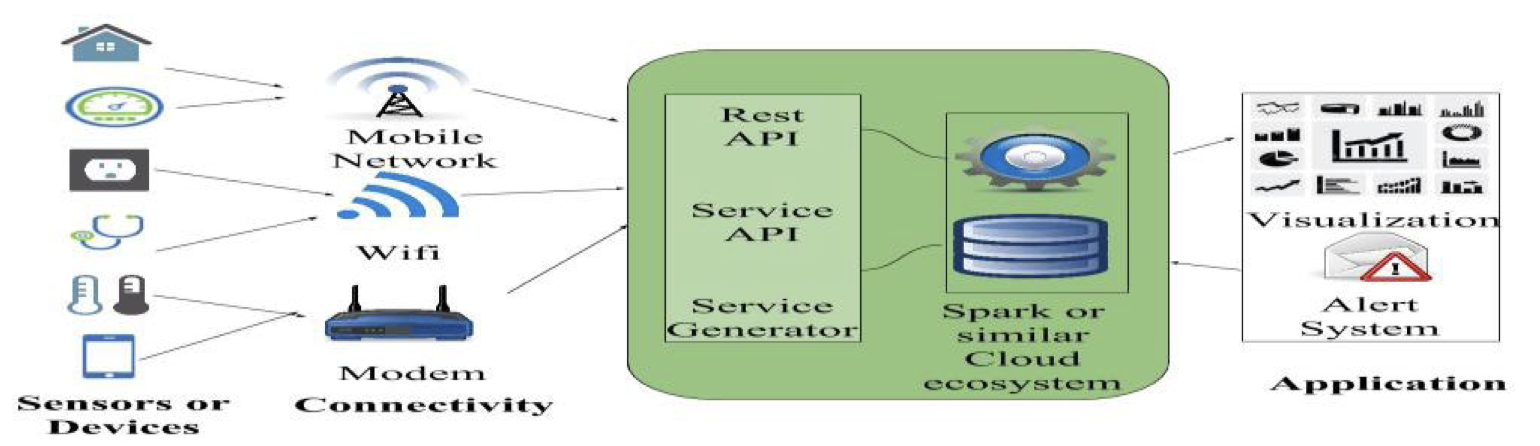
\includegraphics[width=13 cm]{imatges/firstIoTFramework.png}
\caption{\label{fig:firstIoTFramework} First published  framework for an IoT System in this scope by ~\cite{vijai2016design}.}
\end{figure}

A professor at the Politecnico di Torino in 2017 proposed SPEC (Scalable Predictor of Energy Consumption) distributed and parallel approaches "accompanied with cloud-based services (e.g. Platform-as-a-Service tools) due to the increasing volume of collected data as well as the horizontal scaling in hardware"~\cite{cerquitelli2017predicting}. 

Their datasets were "stored in a cluster at our University running Cloudera Distribution of Apache Hadoop (CDH5.3.1). All experiments have been performed on our cluster, which has 8 worker nodes and runs Spark 1.2.0, HDFS 2.5.0, and Yarn 2.5.0. The current implementation of SPEC is a project developed in Scala exploiting the Apache Spark framework"~\cite{cerquitelli2017predicting}. 

\begin{figure}[]
\centering
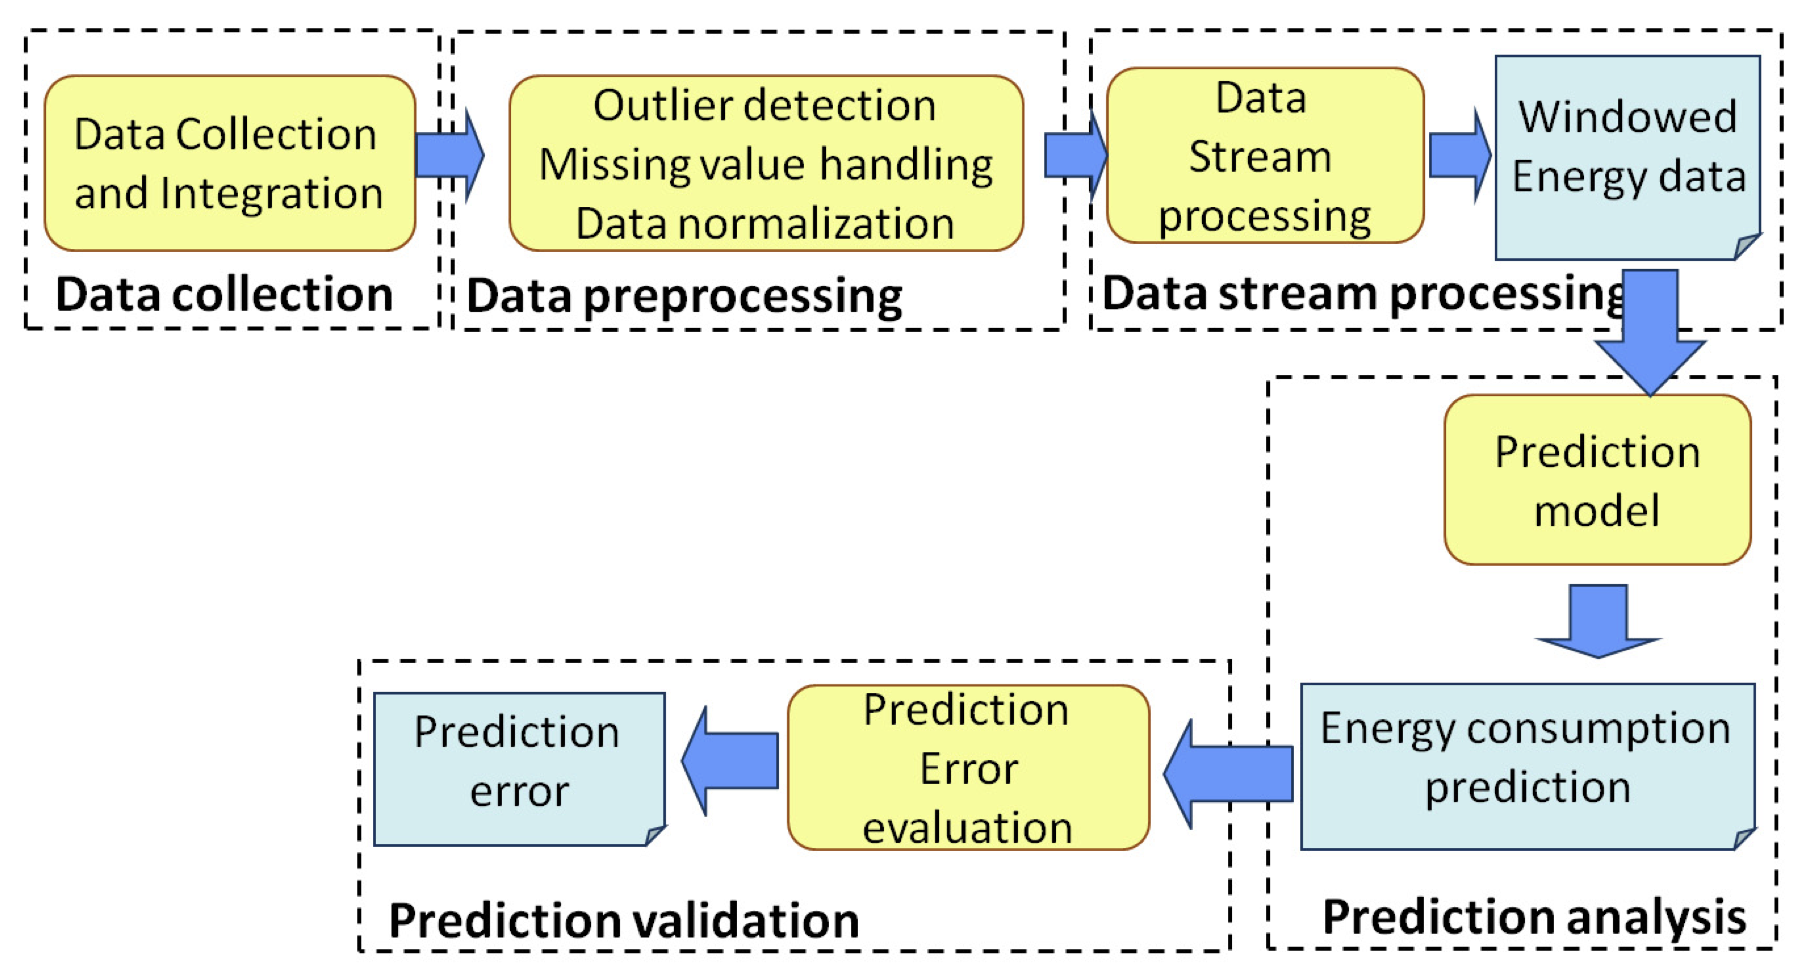
\includegraphics[width=13 cm]{imatges/SPECarchitecture.png}
\caption{\label{fig:SPECarchitecture} SPEC architecture energy-related applications by ~\cite{cerquitelli2017predicting}.}
\end{figure}

In figure~\ref{fig:SPECarchitecture} there is the architecture that she proposes that includes the processing of a window of 5 minutes that provides a glance of the most recent energy usage data that was recorded. It delivers a breakdown of the building's recent past energy consumption and, as a result, forecasts the building's upcoming energy needs in the near future. Researchers who replicated this architecture are ~\cite{Wang2017Taxis}, ~\cite{liu2018scalable}, ~\cite{bangui2021hybrid}, ~\cite{leiria2021using}, ~\cite{abd2022analyze}, ~\cite{ali2020data}, ~\cite{hangan2022advanced}, ~\cite{saheed2022machine}, ~\cite{bukhari2023anomaly}, ~\cite{yadav2023augmentation}, ~\cite{wu2023gtfs}.

Researchers from the Technical University of Denmark in 2018 acknowledge and name for the very first time a \textit{Lambda Architecture} (figure~\ref{fig:lambdaArchitecture}).

\begin{figure}[hbt]
\centering
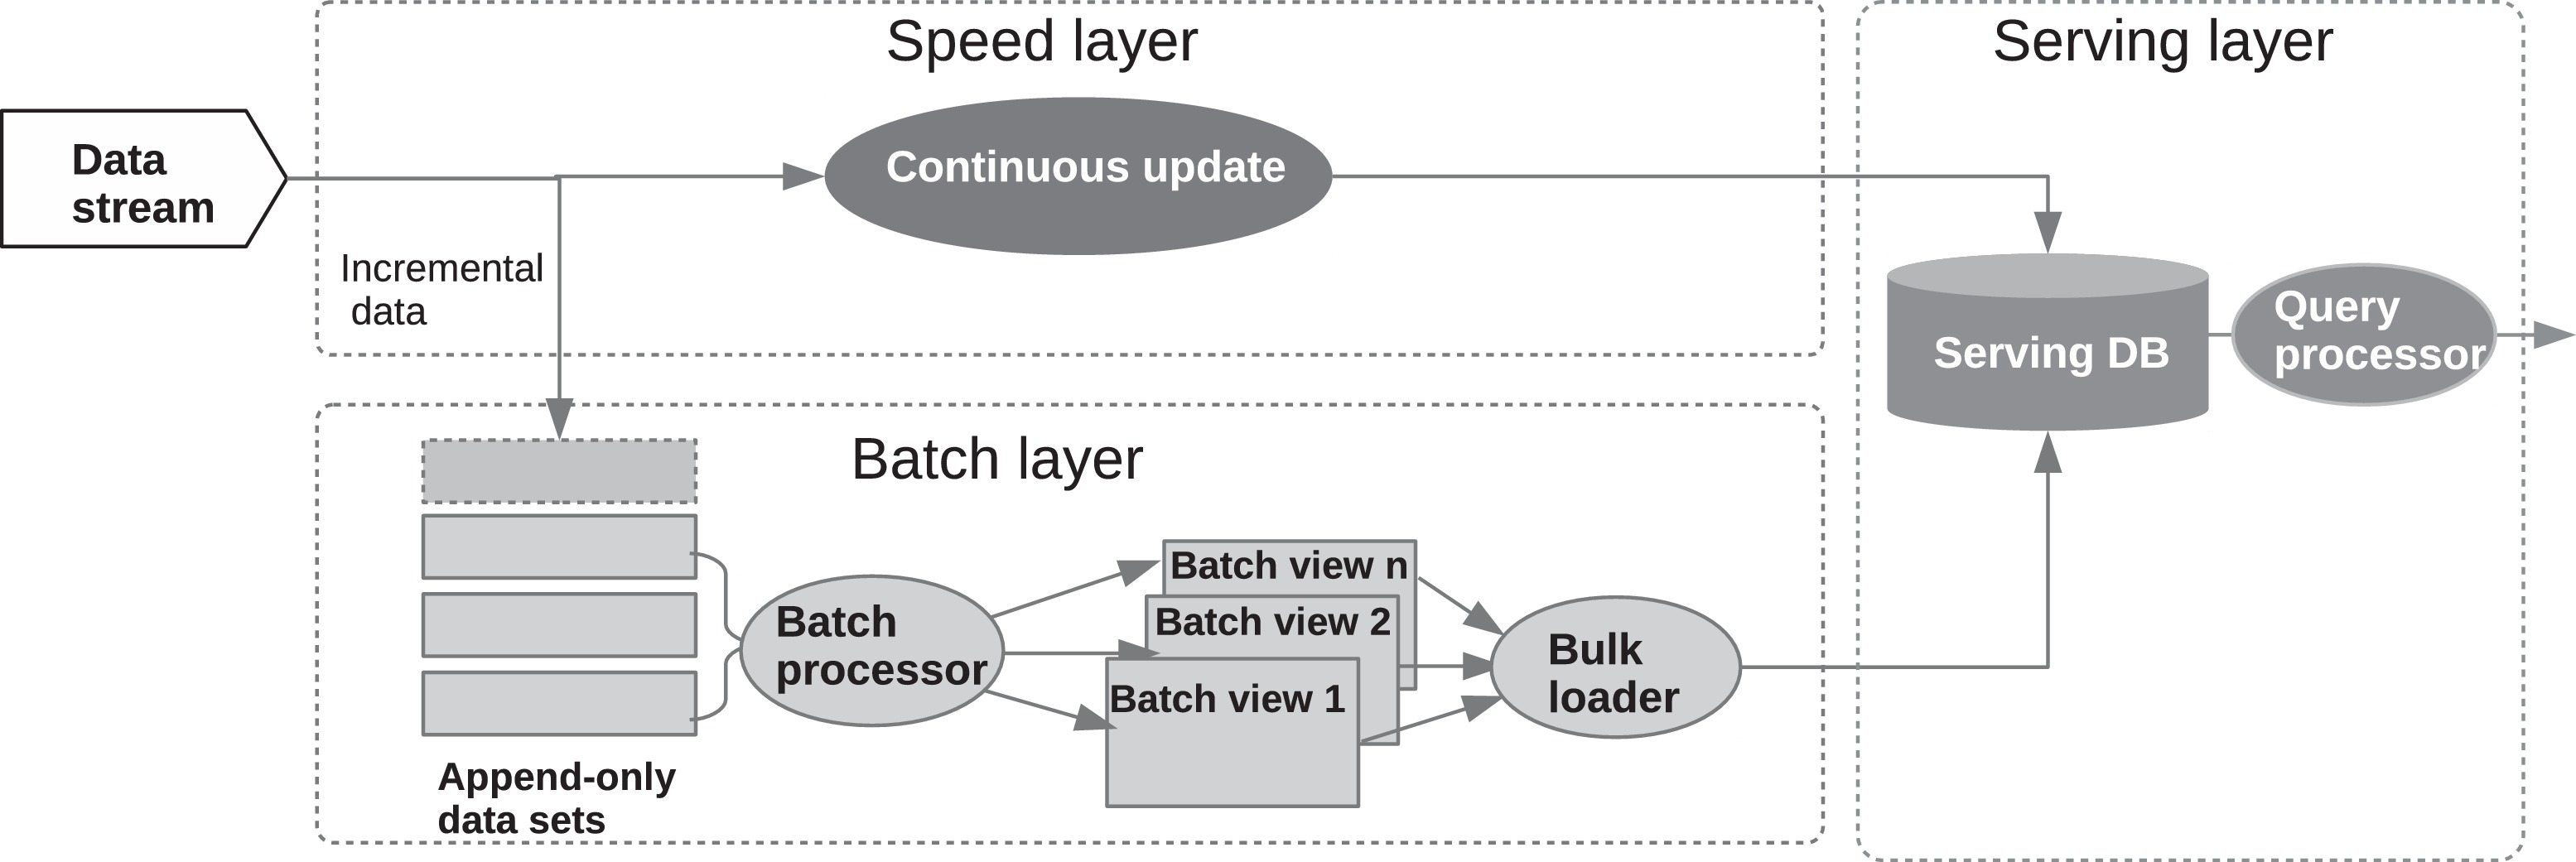
\includegraphics[width=13 cm]{imatges/lambdaArchitecture.jpeg}
\caption{\label{fig:lambdaArchitecture} Lambda Architecture in ~\cite{liu2018scalable}.}
\end{figure}

\textit{"In a lambda system, the data pipeline is broken down into the three layers with clear demarcation of responsibilities. For each layer, there are different technologies that can be used for the implementation. The speed layer performs low-latency computations for incremental data. The streaming technology, such as Spark Streaming, Storm or S4, can be applied to this layer. The batch layer does batch computations for entire data sets, which requires good scalability. The big data processing systems, such as Spark, Hadoop, Pig, and Hive, are the good candidates for this layer. The serving layer needs to respond user queries quickly, which requires a high-performance system. The technologies, including traditional relational data management system (RDBMS), memory-based data stores (Redis or Memcache), are NoSQL database systems (Cassandra, MongoDB, or HBase), are the good options"}~\cite{liu2018scalable}.

In 2019, scholars from the University of Ottawa, Canada, and Harbin University of Science and Technology,  China, proposed an improved lambda architecture (figure~\ref{fig:killenArchitecture}). This time it describes what happens on the 3 layers depending on the latency. The \textit{Perception Layer} acquires and gathers the data to send it and store it in the \textit{Middleware Layer}, and then examines it in the \textit{Application Layer}. 

\begin{figure}[hbt]
\centering
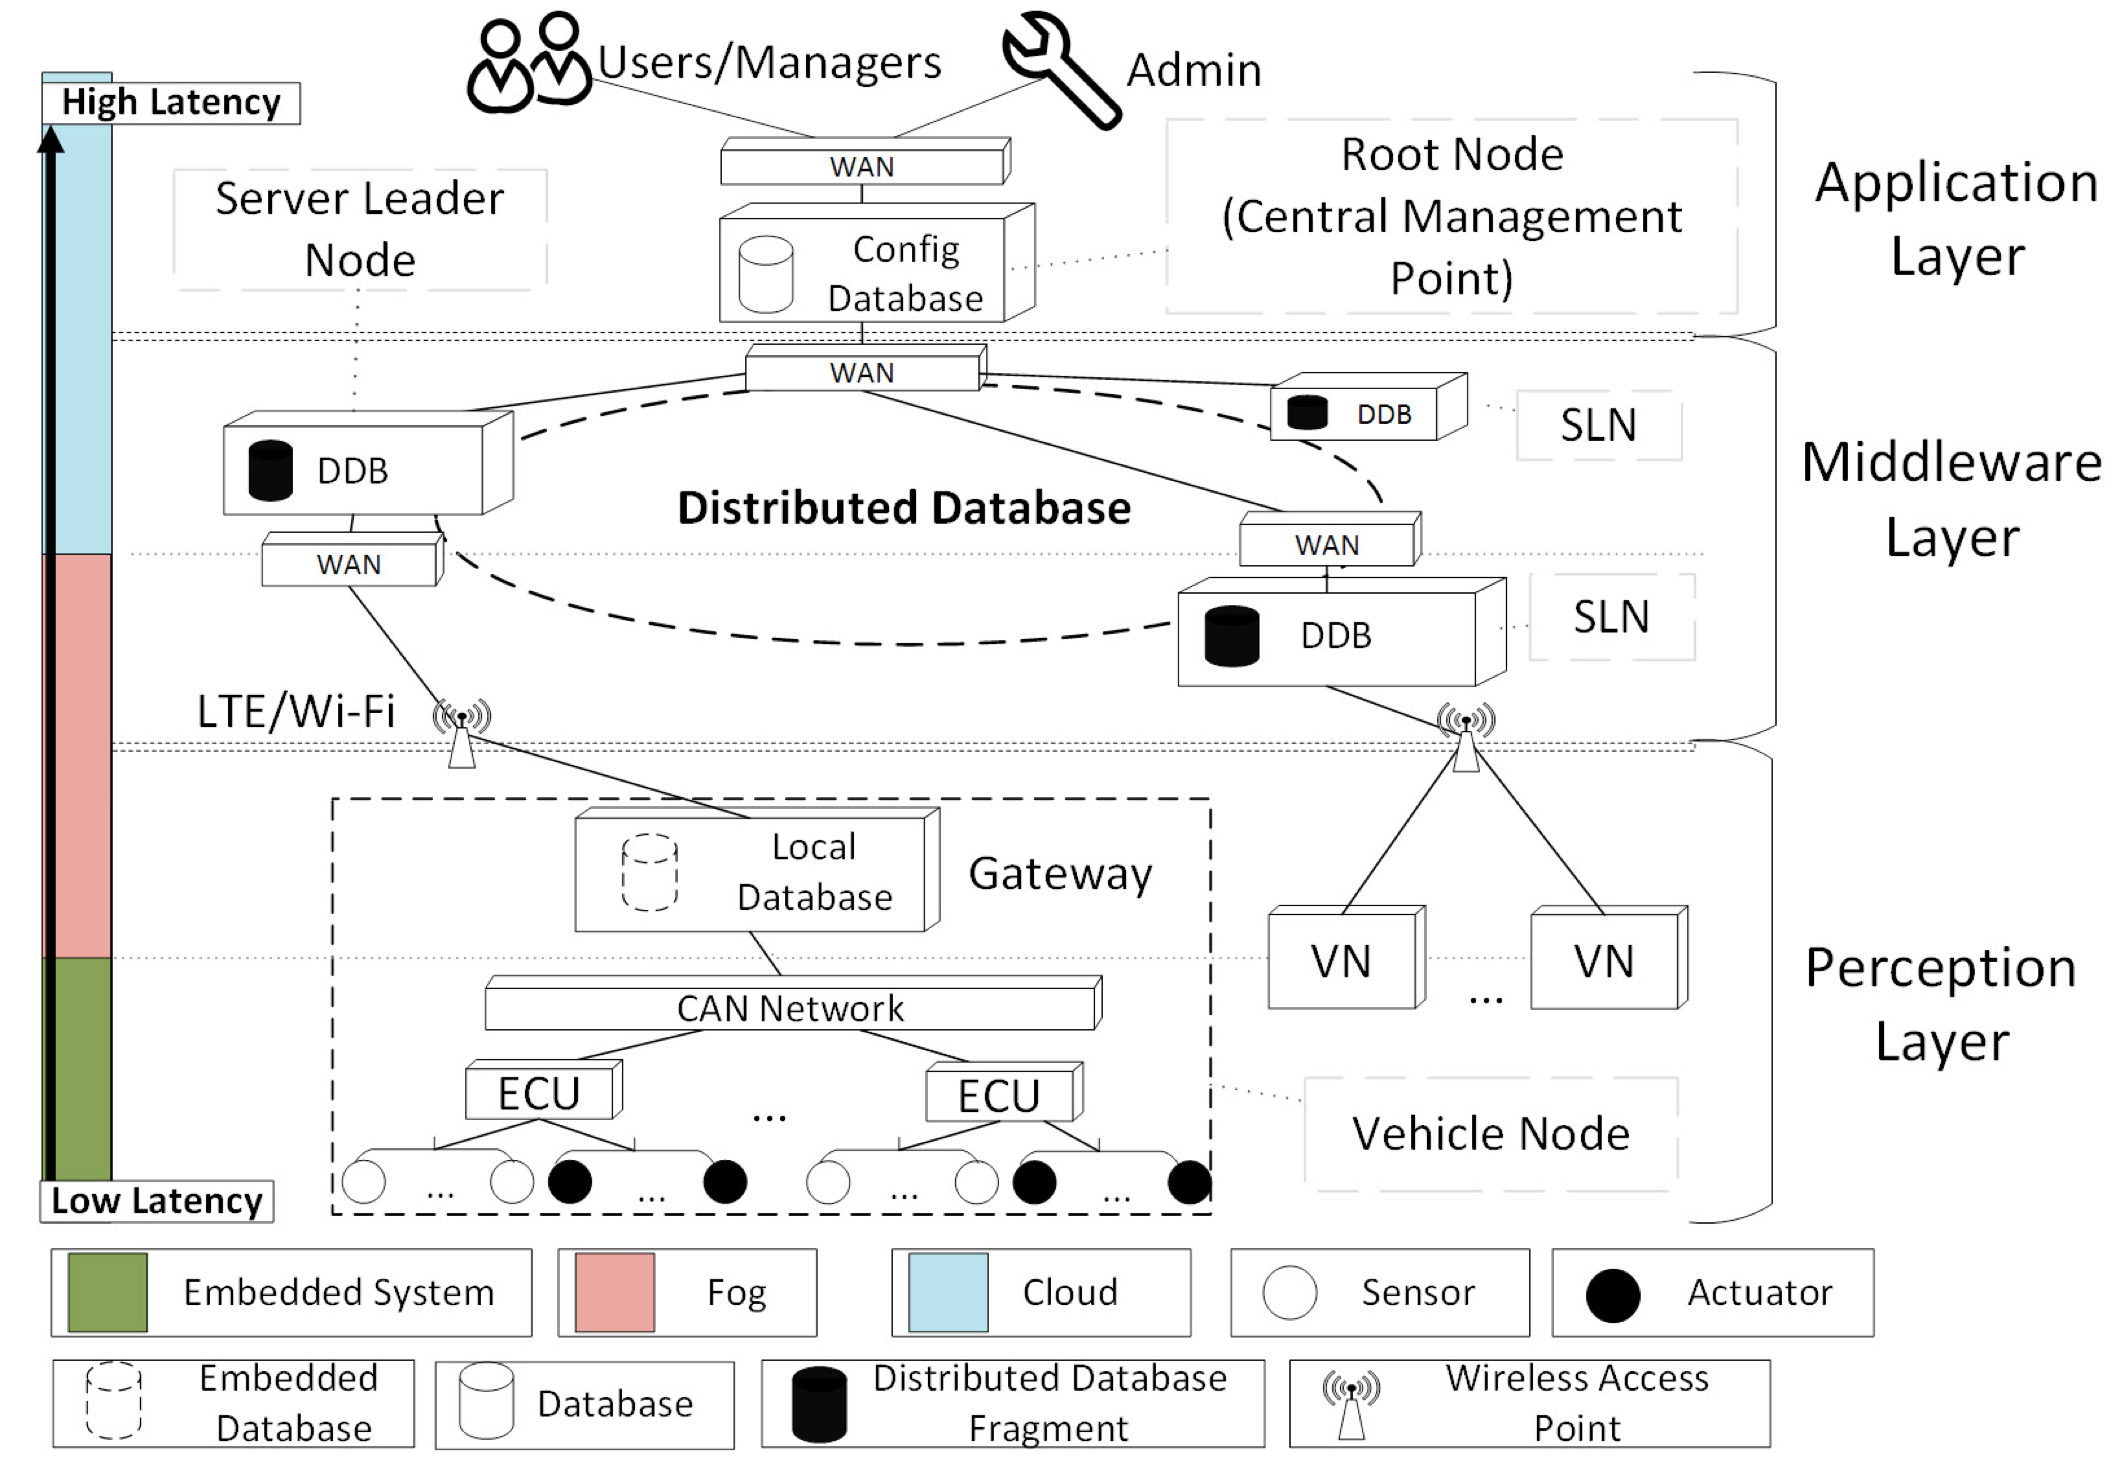
\includegraphics[width=13 cm]{imatges/killenArchitecture.png}
\caption{\label{fig:killenArchitecture} Predictive maintenance fleet management system architecture-overview diagram by ~\cite{killeen2019iot}.}
\end{figure}

\subsection{Data engineering}
\label{section:dataengineering}

Most of the publications that have referred to the data engineering of a smart city are published by \textit{IEEE} and have been studied in the area of \textit{Transportation} (table~\ref{taula:PDEngineering}). 

\renewcommand{\arraystretch}{1.5}
\begin{longtable}{  l l l  }
\caption{Papers related to data engineering.}  \\
\label{taula:PDEngineering}  \\
\hline
  \textbf{Area of study} & \textbf{Journal} & \textbf{Paper} \\
\hline 
\endfirsthead
 \hline
  \textbf{Area of study} & \textbf{Journal} & \textbf{Paper} \\
\hline 
\endhead
\hline
\endfoot
\multirow{6}{*}{CyberSecurity} & \multirow{1}{*}{\textit{Procedia Computer Science}} &   ~\cite{bukhari2023anomaly} \\
 \cline{2-3} 
 & \textit{Measurement: Sensors} &  ~\cite{abd2022analyze} \\
\cline{2-3} 
 & \textit{Electronics} &  ~\cite{protic2022cybersecurity} \\
 \cline{2-3} 
  & \multirow{2}{*}{\textit{Alexandria Engineering Journal}} &  ~\cite{saheed2022machine} \\
 &  &  ~\cite{yadav2023augmentation} \\
\hline
\multirow{5}{*}{Energy}  & \multirow{2}{*}{\textit{Energy Procedia}} &  ~\cite{cerquitelli2017predicting} \\
 & &  ~\cite{du2019clustering} \\
\cline{2-3} 
 & \textit{Applied Energy} &  ~\cite{ali2020data} \\
\cline{2-3} 
  & \parbox{5.5cm}{\textit{Sustainable Energy Technologies and Assessments}} &  ~\cite{moon2022toward} \\
\cline{2-3} 
 & \textit{Environmental Challenges} &  ~\cite{alsalemi2023modular} \\
\hline
\multirow{2}{*}{Environment}  & \textit{IEEE} &  ~\cite{Carbone2017heating} \\
\cline{2-3} 
 & \textit{Water} & ~\cite{hangan2022advanced} \\
\hline
\multirow{1}{*}{People} & \multirow{1}{*}{\textit{IEEE}} & ~\cite{Zhu2020cellular}  \\
\hline 
\multirow{1}{*}{Structures}  & \textit{IEEE} & ~\cite{Zinno2022bridges} \\
\hline
\multirow{7}{*}{Transportation}  &  \multirow{5}{*}{\textit{IEEE}} & ~\cite{Wang2017Taxis}  \\
  &  & ~\cite{Zhao2017passenger}  \\
  &  & ~\cite{Bawaneh2019traffic}  \\
  &  & ~\cite{Nugraha2021rail}  \\
  &  & ~\cite{Wang2021CAN}  \\
 \cline{2-3} 
 & \textit{Big Data Research} & ~\cite{bachechi2022big}  \\
 \cline{2-3} 
 & \parbox{5cm}{\textit{International Journal of Transportation Science and Technology}} & ~\cite{wu2023gtfs}  \\
\end{longtable}

To perform some data engineering, first, there needs to be some data cleaning, as it is necessary given that the raw data frequently has unrelated data and missing data (which could lead to anomalies)~\cite{Bawaneh2019traffic},~\cite{du2019clustering},~\cite{Nugraha2021rail},~\cite{bachechi2022big},~\cite{hangan2022advanced}. That would "assure data accuracy by searching for duplicated or unrealistic information"~\cite{yadav2023augmentation}. According to ~\cite{cerquitelli2017predicting} and~\cite{abd2022analyze}, extreme values, also known as outliers, are not included in the training dataset, despite the fact that they are necessary for the anomaly identification method.

Subsequently, since it "helps to eliminate defects in the dataset"~\cite{saheed2022machine}. One way to do it would be by using a feature scaling approach known as normalization to scale all of the attribute values to the same scale. Standardized moment, z-score normalization, and min-max normalization are a few examples of these techniques~\cite{Carbone2017heating}.

A key for data reduction is selecting solely the essential features that are capable of meeting the needs of the model in order to decrease overfitting and increase accuracy~\cite{Wang2017Taxis},~\cite{ali2020data},~\cite{protic2022cybersecurity},~\cite{alsalemi2023modular}. A threshold limit is chosen for the datasets using information gain as the foundation in order to choose the features. Information gathering that goes beyond a certain point is always a must for accurately identifying cyberattacks~\cite{bukhari2023anomaly}. 

\begin{figure}[hbt]
\centering
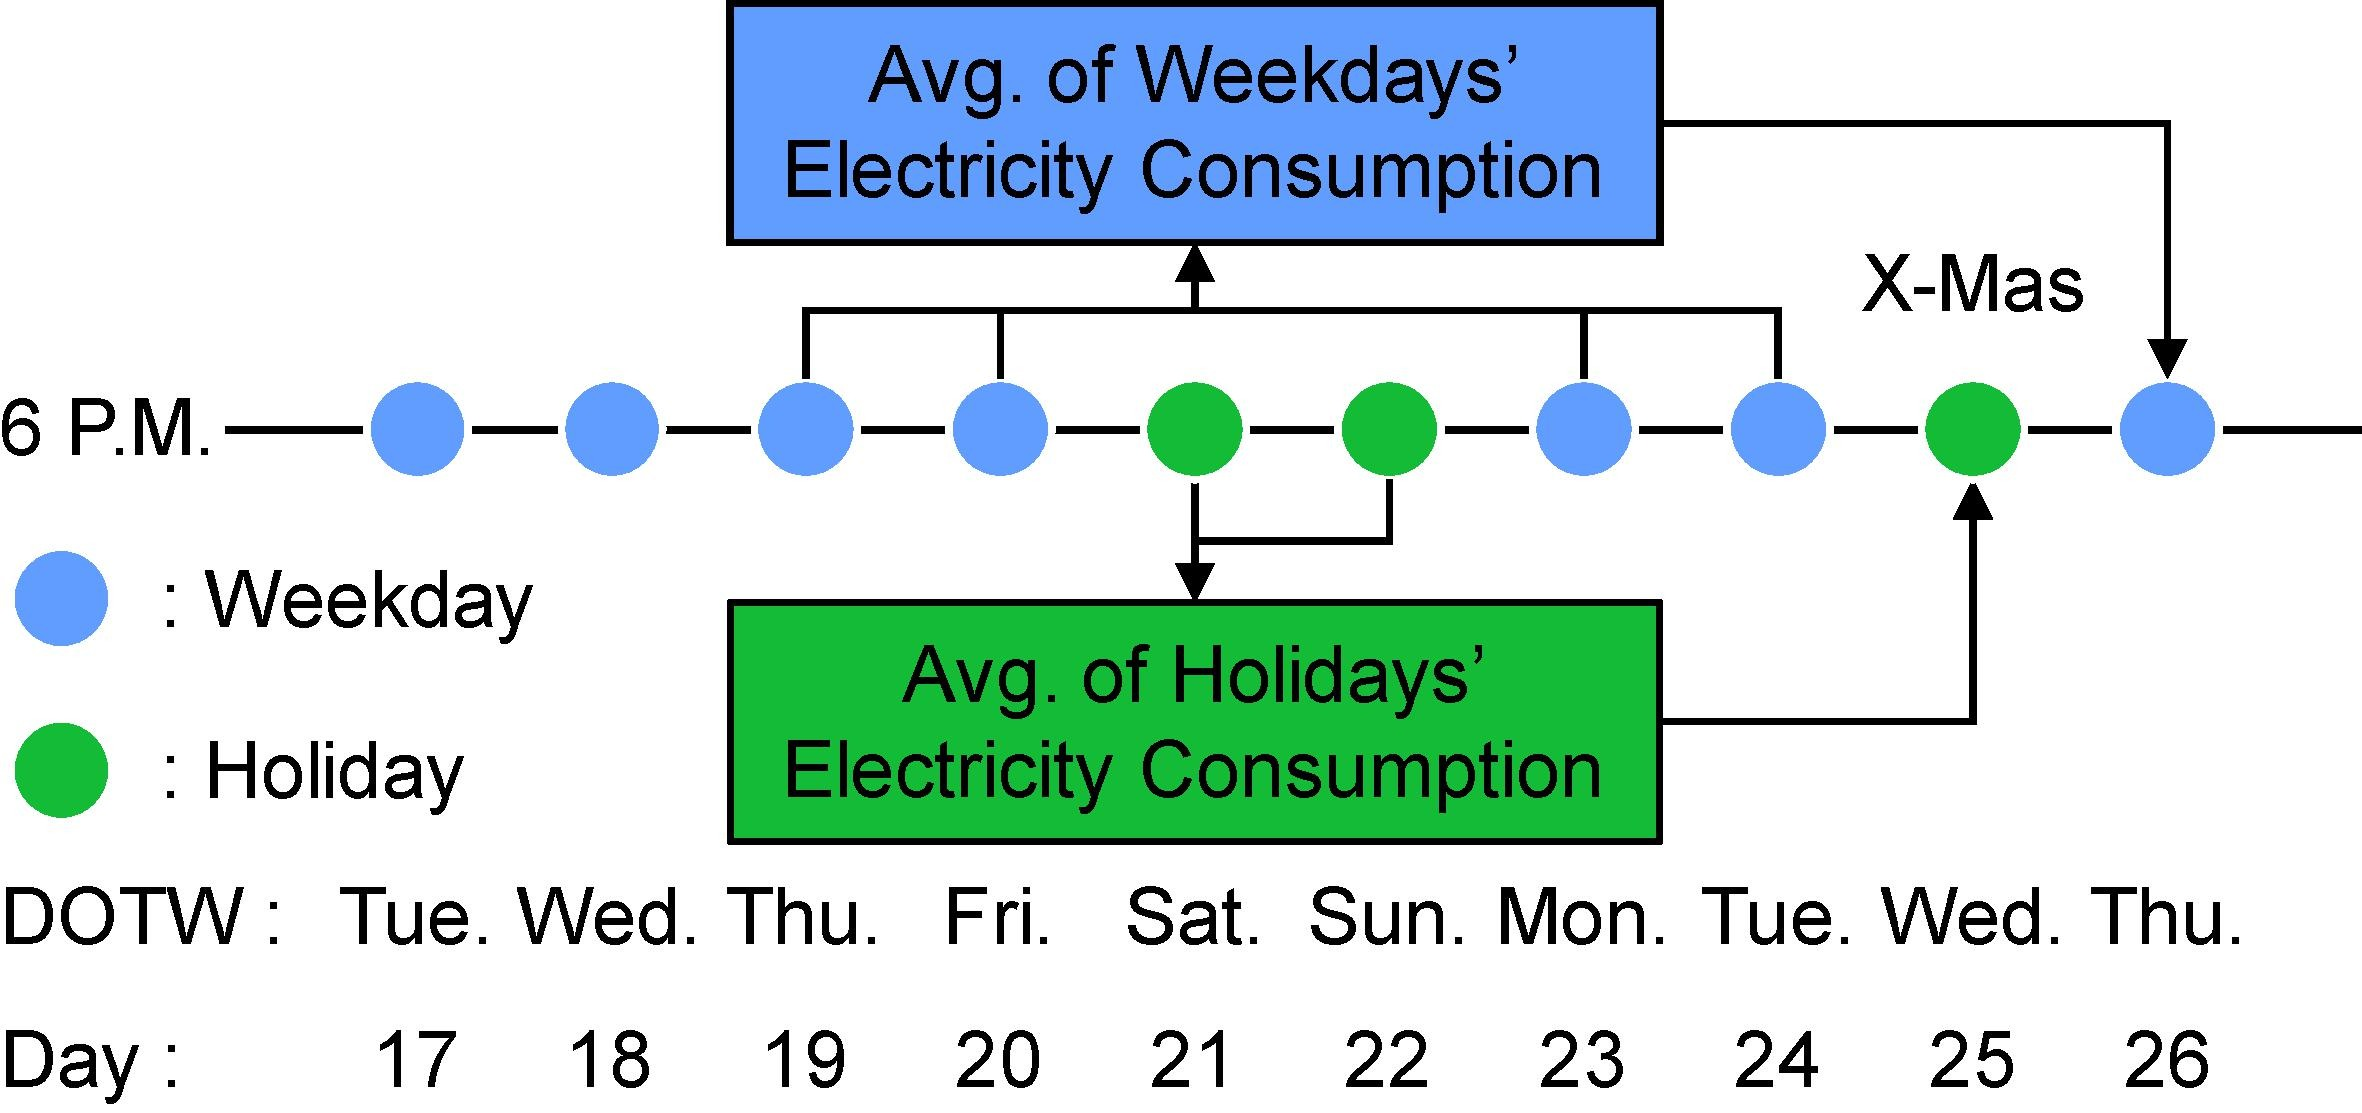
\includegraphics[width=13 cm]{imatges/calendarMoon.jpeg}
\caption{\label{fig:calendarMoon} Example of the weekly average electricity consumption calculation (December 2019). DOTW: days of the week; X-Mas: Christmas. By ~\cite{moon2022toward}.}
\end{figure}

Data integration/fusion is the process of combining data from different sources. It could be used to also transform the current variables or add new ones~\cite{Zhao2017passenger},~\cite{ali2020data},~\cite{Wang2021CAN},~\cite{Zinno2022bridges},~\cite{wu2023gtfs}. For example: a calendar with holidays that happen on specific days that could alter the trending pattern (figure~\ref{fig:calendarMoon}).

Finally, data discretization "replaces numerical attributes with nominal values"~\cite{ali2020data}. Equally important, to avoid data sparsity, you can sum values up to a single value that describes the total activity generated by a category~\cite{Zhu2020cellular}. 

\section{Predictive models}
\label{subcap:predictivemodels}

Anomalies come in many forms, including cyber assaults, data quality, and data values. Consequently, to predict it will change from one anomaly to another. In addition, it could also have a different approach depending on the data. It could perform Supervised or Unsupervised ML.

\begin{figure}[htb]
\centering

\includegraphics[width=13 cm]{imatges/modelsDB.png}
\caption{\label{fig:modelsDB} Models studied on the reviewed papers.}
\end{figure}

In figure~\ref{fig:modelsDB}, there are the models mentioned in the reviewed, and figure~\ref{fig:shareModelsDB} shows the share of the frequency that kind of ML approach was utilized. 

\begin{figure}[htb]
\centering
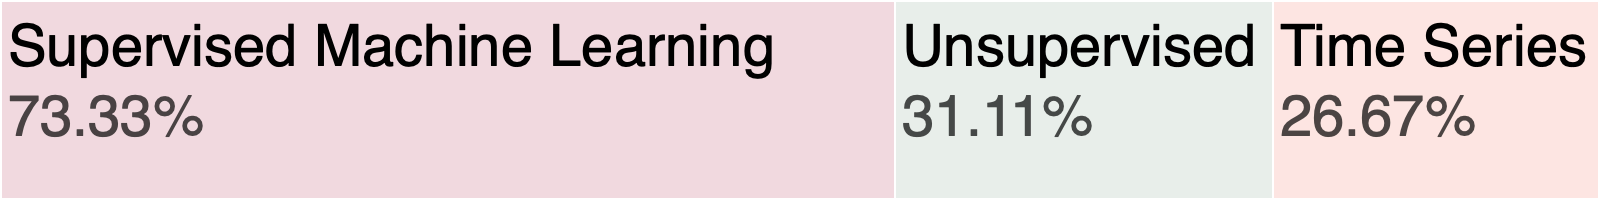
\includegraphics[width=13 cm]{imatges/shareModelsDB.png}
\caption{\label{fig:shareModelsDB} Share of type of machine learning models used on the reviewed papers.}
\end{figure}

\subsection{Supervised Machine Learning}

Most of the publications that have referred to Supervised ML to detect anomalies are classification models like KNN, SVM, and RF. They have been studied the most in the area of \textit{Transportation} (table~\ref{taula:PSMLM}). 

The only regressions that were performed were \textit{Linear Regression}, one in road traffic~\cite{mondal2020road} and one in energy consumption~\cite{leiria2021using}. 

\renewcommand{\arraystretch}{1.5}
\begin{longtable}{  l  c  c  l  }
\caption{Papers related to supervised ML models.}  \\
\label{taula:PSMLM}  \\
\hline
  \textbf{Area of study} & \textbf{Class} & \textbf{Approach} & \textbf{Paper} \\
\hline 
\endfirsthead
 \hline
  \textbf{Area of study} & \textbf{Class} & \textbf{Approach} & \textbf{Paper} \\
\hline 
\endhead
\hline
\endfoot
\multirow{8}{*}{CyberSecurity} & \multirow{8}{*}{Classification}  & RF & ~\cite{saranya2020performance} \\
\cline{3-4} 
 &  & \multirow{3}{*}{SVM} & ~\cite{el2014multicriterion} \\
 &  &  & ~\cite{Xu2019outlier}\\
 &  &  & ~\cite{bukhari2023anomaly}\\
 \cline{3-4} 
 &  & KNN & ~\cite{protic2022cybersecurity} \\
 \cline{3-4} 
 &  & \multirow{3}{*}{XGBoost} & ~\cite{karanfilovska2022analysis} \\
  &  & & ~\cite{saheed2022machine} \\
  &  & & ~\cite{yadav2023augmentation} \\
\hline
\multirow{6}{*}{Energy} & \multirow{5}{*}{Classification}  & GBoost & ~\cite{ali2020data} \\
\cline{3-4} 
 &  & KNN & ~\cite{himeur2020data} \\
 \cline{3-4} 
 &  & LightGBM & ~\cite{moon2022toward} \\
 \cline{3-4} 
 &  & RF & ~\cite{cerquitelli2017predicting} \\
 \cline{3-4} 
 &  & RS & ~\cite{alsalemi2023modular} \\
 \cline{2-4} 
 & Regression  & Linear Regression & ~\cite{leiria2021using} \\
 \hline
\multirow{1}{*}{Environment} & \multirow{1}{*}{Classification}  & KNN & ~\cite{hangan2022advanced} \\
\hline
Structures & Classification  & RF & ~\cite{Zinno2022bridges} \\
\hline
People & Classification & RS & ~\cite{embarak2021new} \\
\hline
\multirow{6}{*}{Transportation} & \multirow{6}{*}{Classification}  & Bayesian Model & ~\cite{vidovic2022methodology}  \\
\cline{3-4} 
 & & COSMO & ~\cite{killeen2019iot}  \\
 \cline{3-4} 
 & & K-D tree & ~\cite{masino2017learning} \\
  \cline{3-4} 
 &  & Logical Regression & ~\cite{Wang2017Taxis} \\
 \cline{3-4} 
 & & RUSBoost & ~\cite{kyriakou2021vehicles} \\
 \cline{3-4} 
 & & \multirow{1}{*}{SVM} & ~\cite{Wang2017Taxis} \\
 \multirow{5}{*}{Transportation} & \multirow{3}{*}{Classification} & \multirow{3}{*}{SVM} & ~\cite{zantalis2019review} \\
 & & & ~\cite{sara2020predict} \\
 & & & ~\cite{Nugraha2021rail} \\
 \cline{3-4} 
 & & XGBoost & ~\cite{Wang2021CAN} \\
 \cline{2-4} 
 & \multirow{1}{*}{Regression} & Linear Regression & ~\cite{mondal2020road} \\
\end{longtable}

\renewcommand{\arraystretch}{1.5}
\begin{landscape}
\begin{longtable}{  l  c  c  l  }
\caption{Findings on papers related to supervised ML models.}  \\
\label{taula:PSMLM}  \\
 \hline
  \textbf{Citation} & \textbf{Area of study} & \textbf{Approach} & \textbf{Findings}  \\
\hline 
\endfirsthead
 \hline
  \textbf{Citation} & \textbf{Area of study} & \textbf{Approach} & \textbf{Findings}  \\
\hline 
\endhead
\hline
\endfoot
\\
\parbox{1.5cm}{~\cite{el2014multicriterion}}  & CyberSecurity & SVM & \parbox{12cm}{It explores a new countermeasure approach for anomaly-based intrusion detection using a multicriterion fuzzy classification method combined with a greedy attribute selection.} \\
\\
\parbox{1.5cm}{~\cite{cerquitelli2017predicting}}  & Energy & RF & \parbox{12cm}{The preliminary version of the SPEC (Scalable Predictor of Energy Consumption) engine to address the fine grain prediction of energy consumption over a sliding time window.} \\
\\
\parbox{1.5cm}{~\cite{masino2017learning}} & Transportation & K-D tree & \parbox{12cm}{The results show that the method and Euclidean distance performs best and is robust in transferring the information of the road surface from one vehicle to another.} \\
\\
\parbox{1cm}{~\cite{Wang2017Taxis}}  & \parbox{2.5cm}{Transportation} & \parbox{2.2cm}{Logical Regression (LR) and SVM} & \parbox{12cm}{LR outperforms SVM and decision trees in prediction accuracy and F-score measurement, while SVM is capable of identifying the largest number of unlicensed taxis. The model's learning phase can be improved even further with other heterogeneous datasets like demographics, sites of interest, etc.} \\
\\
\parbox{1cm}{~\cite{killeen2019iot}}  & Transportation & \parbox{3cm}{Consensus self-organized models approach (COSMO)} & \parbox{12cm}{It proposes a novel IoT architecture for predictive maintenance and proposes a semi-supervised machine learning algorithm that attempts to improve the sensor selection performed in a predictive maintenance system.} \\
\\
\parbox{0.5cm}{~\cite{Xu2019outlier}} & CyberSecurity & One Class SVM & \parbox{12cm}{The predictive performance of the tuned Local Outlier Factor is comparable to the predictive performance with the best results on the Http and Smtp data, and it outperforms all the other methods on Credit and Mnist data.} \\
\\
\parbox{1.7cm}{~\cite{zantalis2019review}} & Transportation & SVM & \parbox{12cm}{Given the current applications and infrastructure regarding IoT and ML, a comparatively smaller ML coverage for the smart lighting systems and parking applications are detected.} \\
\\
\parbox{0.5cm}{~\cite{ali2020data}}  & Energy & \parbox{3cm}{Gradient Boosted trees} & \parbox{12cm}{It extracts the knowledge from available resources to identify the existing building energy performance and formulate retrofit solutions.} \\
\\
\parbox{1cm}{~\cite{himeur2020data}}  & Energy & KNN & \parbox{12cm}{They discussed the usefulness of several data fusion strategies that have been implemented or could be deployed to decrease energy wastage and promote sustainability.} \\
\\
\parbox{1cm}{~\cite{sara2020predict}}  & Transportation & SVM and RF & \parbox{12cm}{While training the SVM had a better accuracy score than the RF. However, test results are better than the SVM.} \\
\\
\parbox{1.6cm}{~\cite{mondal2020road}}  & Transportation & \parbox{3.2cm}{Linear Regression} & \parbox{12cm}{It proposes a technique based on a statistical model which identifies the temporal outliers. It can be used to detect unusual traffic incidents or sensor failures.} \\
\\
\parbox{1.85cm}{~\cite{embarak2021new}}  & People & \parbox{3cm}{RS} & \parbox{12cm}{All proposed solutions fell within the scope of predictions that result in active or proactive actions to support universities and learners. On the other hand, they fail to comprehend the various forms of education systems and whether it appropriate for the twenty-first century and future generations.} \\
\\
\parbox{1.7cm}{~\cite{saranya2020performance}}  & CyberSecurity & RF & \parbox{12cm}{It conveys that the detection rate, false positive rate, and accuracy not only depend on the algorithm but also depend on the application area.} \\
\\
\parbox{1.85cm}{~\cite{kyriakou2021vehicles}}  & Transportation & \parbox{3.2cm}{RUS Boosted trees} & \parbox{12cm}{It has already been field-tested for the detection and classification of cracks, rutting, ravelling, patches and potholes, exhibiting accuracy levels higher than 90\%.} \\
\\
\parbox{1cm}{~\cite{leiria2021using}}  & Energy & \parbox{3.2cm}{Linear Regression} & \parbox{12cm}{They analyze measured variables (heat consumption, outdoor temperature, wind speed, and global radiation) to acquire new knowledge on the building characteristics.} \\
\\
\parbox{1.8cm}{~\cite{Nugraha2021rail}}  & Transportation & \parbox{3cm}{One Class SVM} & \parbox{12cm}{To accurately predict the condition of critical components, it can be started with data collection, followed by detecting normal and abnormal behavior, and continued by training algorithms to make predictions.} \\
\\
\parbox{1cm}{~\cite{Wang2021CAN}}  & Transportation & \parbox{2.2cm}{Focal Loss - XGBoost} & \parbox{12cm}{For the case of sample imbalance, the model has a high accuracy rate in resisting tampered data domain messages.} \\
\\
\parbox{1cm}{~\cite{hangan2022advanced}}  & Environment & KNN & \parbox{12cm}{The model calculates an anomaly score for each day, based on ten features of daily demand and its historical context. The authors use calendar contexts within the anomaly detection algorithm. A calendar context for a day d is a subset of days from the database D that would be expected to have similar water use as d. This allows them to give possible causes for the detected anomalies. The score and its explanations are posted to users to help them track down the physical causes of anomalies.} \\
\\
\parbox{2.65cm}{~\cite{karanfilovska2022analysis}}  & CyberSecurity & XGBoost & \parbox{12cm}{Using the approach with StandardScalerWrapper achieved in Azure AML tool, it can be said that machine learning is very applicable in solving anomaly detection problems in IoT networks. This was also shown with the experiments performed with the AE2EML tool, which have resulted with F-Score greater than 95\%} \\
\\
\parbox{1cm}{~\cite{moon2022toward}}  & Energy & LightGBM & \parbox{12cm}{They confirmed that the Temperature-Humidity Index (THI) and the Wind Chill Index (WCT) exhibited more influence on forecasting model construction than temperature, humidity, and wind speed in weather information. Because the Shapley additive explanations value was large for THI in summer and WCT in winter, they estimated that they contribute to more accurate day-ahead hourly electricity consumption forecasting for summer and winter, respectively.} \\
\\
\parbox{1.3cm}{~\cite{protic2022cybersecurity}}  & CyberSecurity & Weighted KNN & \parbox{12cm}{The results show a clear benefit of the Tangent-Hyperbolic  normalization used for scaling regarding processing time. Regardless of how accurate the classifiers are, their decisions can sometimes differ.} \\
\\
\parbox{1.6cm}{~\cite{saheed2022machine}}  & CyberSecurity & XGBoost & \parbox{12cm}{They performed a dimensionality reduction with Principal Component Analysis (PCA). They infer that using machine learning techniques for successful anomaly detection in the IoT environment is both realistic and practicable.} \\
\\
\parbox{1.6cm}{~\cite{vidovic2022methodology}}  & Transportation & \parbox{3cm}{Bayesian Model} & \parbox{12cm}{The model when paired with additional data sets (e.g. public transport timetables, location of public transport stations, information on public transport lines, etc.), it can be used for modal split detection.} \\
\\
\parbox{1cm}{~\cite{Zinno2022bridges}}  & Structures & RF & \parbox{12cm}{Their results showed that less sensors were needed to measure acceleration responses in order to figure out where damage is and how bad it is. Compared to neural network training methods, the proposed method for identifying damage could get good results quickly and with much less computational work and time.} \\
\\
\parbox{1.82cm}{~\cite{alsalemi2023modular}}  & Energy & \parbox{3cm}{RS} & \parbox{12cm}{It presents a modular system for improving domestic household energy savings. It is designed to create customizable sub-components that adapt to the nature of the data and the end-user's preference, such as modules that recommend based on usage patterns, power consumption, and occupancy.} \\
\\
\parbox{1.3cm}{~\cite{bukhari2023anomaly}}  & CyberSecurity & SVM & \parbox{12cm}{ The paper goes on to examine the role of ensemble techniques like bagging and boosting to provide an additional security layer to the detection architecture.} \\
\\
\parbox{1.3cm}{~\cite{yadav2023augmentation}}  & CyberSecurity & XGBoost & \parbox{12cm}{They propose a novel combined feature selection method known as the Fast Correlation-based Feature Selection (FCBFS) with the approach, which can successfully minimize the number of features while maintaining a high classification precision and recognition rate.} \\
\\
\hline
\end{longtable}
\end{landscape}

\subsection{Unsupervised Machine Learning}

Most of the publications that have referred to Unsupervised ML to detect anomalies are clustering models with K-Means. They have been studied the most in the area of \textit{CyberSecurity}, and \textit{Transportation} (table~\ref{taula:PUMLM}). 

There is one paper that tries DBSCAN for on-street parking behavior in Munich~\cite{gomari2021cluster}, and one that uses Dirichlet Mixture for the behavior of wireless networking~\cite{abd2022analyze}.

\renewcommand{\arraystretch}{1.5}
\begin{longtable}{  l  c  l  }
\caption{Papers related to unsupervised ML models.}  \\
\label{taula:PUMLM}  \\
\hline
  \textbf{Area of study} & \textbf{Approach} & \textbf{Paper} \\
\hline 
\endfirsthead
 \hline
  \textbf{Area of study} & \textbf{Approach} & \textbf{Paper} \\
\hline 
\endhead
\hline
\endfoot
\multirow{4}{*}{CyberSecurity} & Dirichlet Mixture & ~\cite{abd2022analyze}  \\
\cline{2-3} 
 & \multirow{3}{*}{K-Means}  & ~\cite{al2018semi}  \\
 &  & ~\cite{bangui2021hybrid}  \\
 &  & ~\cite{karanfilovska2022analysis}  \\
\hline
\multirow{1}{*}{Energy} & \multirow{1}{*}{K-Means}  & ~\cite{du2019clustering}  \\
\hline
\multirow{2}{*}{Environment} & \multirow{2}{*}{K-Means}  & ~\cite{mohamudally2018building}  \\
 &  & ~\cite{hangan2022advanced}  \\
\hline
\multirow{1}{*}{Health} & \multirow{1}{*}{K-Means}  & ~\cite{abu2022automated}  \\
\hline
\multirow{1}{*}{People} & K-Means & ~\cite{Zhu2020cellular}  \\
\hline
Structures & Fuzzy C-Means & ~\cite{Zinno2022bridges}  \\
\hline
\multirow{4}{*}{Transportation} & \multirow{1}{*}{DBSCAN}  & ~\cite{gomari2021cluster}  \\
\cline{2-3} 
 & \multirow{3}{*}{K-Means}  & ~\cite{Zhao2017passenger}  \\
 &  & ~\cite{belhadi2020space}  \\
 &  & ~\cite{gomari2021cluster}  \\
\end{longtable}

\renewcommand{\arraystretch}{1.5}
\begin{landscape}
\begin{longtable}{  l  c  c  l  }
\caption{Findings on papers related to unsupervised ML models.}  \\
\label{taula:PUMLM}  \\
 \hline
  \textbf{Citation} & \textbf{Area of study} & \textbf{Approach} & \textbf{Findings}  \\
\hline 
\endfirsthead
 \hline
  \textbf{Citation} & \textbf{Area of study} & \textbf{Approach} & \textbf{Findings}  \\
\hline 
\endhead
\hline
\endfoot
\\
\parbox{0.5cm}{~\cite{Zhao2017passenger}}  & Transportation & K-Means & \parbox{12.5cm}{They looked into the passenger travel distribution patterns and find out the abnormal passengers based on the empirical knowledge. Then, they classified the passengers in terms of the similarity of their travel patterns.} \\
\\
\parbox{1.9cm}{~\cite{al2018semi}}  & CyberSecurity & K-Means & \parbox{12.5cm}{They introduced the use of a weighted Euclidean distance measure based on the observation that different attributes might have a strong impact on the resultant partitions of data. It assigns a weight for each attribute based on its significance in distinguishing between class types. These weighted attributes can lead to a higher probability of obtaining atomic clusters with a lower value of K.} \\
\\
\parbox{2.7cm}{~\cite{mohamudally2018building}}  & Environment & K-Means & \parbox{12.5cm}{The found that ML in the unsupervised mode is indeed very efficient in situations where datasets are unpredictable. Moreover, cases where data points show non-linear time series require multivariate analysis that makes the process more computing-intensive.} \\
\\
\parbox{0.5cm}{~\cite{du2019clustering}}  & Energy & K-Means & \parbox{12.5cm}{Users in the same category do not necessarily have the same energy consumption patterns, which potentially leads to unfair prices and many other practical issues. Their results can serve as potential inputs for future energy price models, demand-side management, and load-reshaping strategies.} \\
\\
\parbox{1.6cm}{~\cite{belhadi2020space}}  & Transportation & K-Means & \parbox{12.5cm}{For each location, they have observed different flow values represented by a time series. Applying space–time series clustering on these data allows the grouping of locations that have similar traffic behaviors. } \\
\\
\parbox{0.5cm}{~\cite{Zhu2020cellular}}  & People & K-Means & \parbox{12.5cm}{This approach can cluster areal units with similar traffic patterns and segment a city into distinct groups. Then, in grouped areas, they detect anomalous behaviors of the cellular network and verify the accuracy of the results using ground truth information collected from online sources.} \\
\\
\parbox{1.6cm}{~\cite{bangui2021hybrid}}  & CyberSecurity & \parbox{2cm}{Weighted K-Means} & \parbox{12.5cm}{They apply the coreset method to deal with computational complexity in clustering and the large volume of vehicular datasets by extracting critical contents without examining all data content, and then enable IDSs to ensure timely network security. This approximate technique is not only just giving a quick viewability of original data, but also helps with scaling Big Data Analytics techniques during data processing.} \\
\\
\parbox{1.6cm}{~\cite{gomari2021cluster}}  & Transportation & \parbox{2cm}{Two-stage: DBSCAN – K-Means} & \parbox{12.5cm}{The method can immediately provide first insights on the spatio-temporal parking behavior that exists within a city while employing a random automated data collection by a fleet of vehicles representing normal human mobility behavior, with a bias towards the group of vehicle users.} \\
\\
\parbox{1.4cm}{~\cite{abd2022analyze}}  & CyberSecurity & \parbox{2.2cm}{Dirichlet Mixture} & \parbox{12cm}{It proposes a hybrid anomaly detection method that combines several characteristic selecting strategies with an appropriate mixture approach to recognize each assault form with great precision.} \\
\\
\parbox{2.35cm}{~\cite{abu2022automated}}  & Health & K-Means & \parbox{12.5cm}{Since the probability of false alarms poses a serious impact on the accuracy of cardiac arrhythmia detection, it is the most important factor to keep false alarms to the lowest level.} \\
\\
\parbox{1cm}{~\cite{hangan2022advanced}}  & Environment & K-Means & \parbox{12.5cm}{They label the clusters according to the predominant peak demand time and discover that patterns that contained multiple peaks during the day were more prone to internal leaks.} \\ 
\\
\parbox{2.65cm}{~\cite{karanfilovska2022analysis}}  & CyberSecurity & K-Means & \parbox{12.5cm}{The results obtained with the PyCaret tool have shown that the silhouette score and distribution of the clusters were improved after applying PCA, while the homogeneity, Rand Index and completeness were better for the clustering without PCA.} \\
\\
\parbox{1cm}{~\cite{Zinno2022bridges}}  & Structures & Fuzzy C-Means & \parbox{12.5cm}{They investigated how vibrations may be utilized to detect deterioration in a truss bridge model and suggested a novel approach based on fuzzy clustering and reduced frequency response function (FRF) data using principal component projection.} \\
\hline
\end{longtable}
\end{landscape}

\subsection{Time Series}

Most of the publications that have referred to Time Series to detect anomalies with SAX model, which has been studied in the areas of \textit{Energy}, and \textit{Environment} (table~\ref{taula:PTSP}). 

\renewcommand{\arraystretch}{1.5}
\begin{longtable}{  l  c  l  }
\caption{Papers related to forecasting time series.}  \\
\label{taula:PTSP}  \\
\hline
  \textbf{Area of study} & \textbf{Approach} & \textbf{Paper} \\
\hline 
\endfirsthead
 \hline
  \textbf{Area of study} & \textbf{Approach} & \textbf{Paper} \\
\hline 
\endhead
\hline
\endfoot
\multirow{3}{*}{Energy}  & SAX & ~\cite{fonseca2017unsupervised}  \\
 \cline{2-3} 
& Average of Heat Loss & ~\cite{gerrish2017analysis}  \\
 \cline{2-3} 
 & PARX & ~\cite{liu2018scalable}  \\
\hline
\multirow{4}{*}{Environment} & Least Square SVM  & ~\cite{vijai2016design}  \\
\cline{2-3} 
 & SAX & ~\cite{Carbone2017heating}  \\
 \cline{2-3} 
 & DTW  & ~\cite{bachechi2022big}  \\
 \cline{2-3} 
 & BSTS  & ~\cite{wu2023gtfs}  \\
\hline
Transportation & OBADA  & ~\cite{Bawaneh2019traffic}  \\
\end{longtable}

\renewcommand{\arraystretch}{1.5}
\begin{landscape}
\begin{longtable}{  l  c  c  l  }
\caption{Findings on papers related to time series predictions.}  \\
\label{taula:PTSP}  \\
 \hline
  \textbf{Citation} & \textbf{Area of study} & \textbf{Approach} & \textbf{Findings}  \\
\hline 
\endfirsthead
 \hline
  \textbf{Citation} & \textbf{Area of study} & \textbf{Approach} & \textbf{Findings}  \\
\hline 
\endhead
\hline
\endfoot
\\
\parbox{1.1cm}{~\cite{vijai2016design}}  & Environment & Least Square SVM & \parbox{12.5cm}{There is a keen interest from the organizations and government to make proper usage of water. The same can be achieved by proper monitoring and management of water distribution systems.} \\
\\
\parbox{1.8cm}{~\cite{Carbone2017heating}}  & Environment & \parbox{3.5cm}{Symbolic Aggregate approXimation (SAX)} & \parbox{12.5cm}{They conjecture that different normalization horizons allow to include in the shape of the time series patterns an additional, variable, component from a longer period trend. To support the analysis phase, a calendar can be used as an additional source of information to discriminate between really unwanted anomalies and expected anomalies (e.g. weekends), or even to signal a possible anomaly whenever a “normal” behavior is not expected.} \\
\\
\parbox{1.7cm}{~\cite{fonseca2017unsupervised}}  & Energy & \parbox{3cm}{Symbolic Aggregate approXimation (SAX)} & \parbox{12.5cm}{ The number of clusters and accuracy of SAX highly depends on the highly sensitive input variables related to size. The approach is subjected to three fitness objectives, i.e., maximize data accuracy and compression and minimize complexity.} \\
\\
\parbox{1.6cm}{~\cite{gerrish2017analysis}}  & Energy & \parbox{3cm}{Average of Heat Loss} & \parbox{12.5cm}{The response of a single space to changing internal and external temperatures can be used to determine whether it responds differently to other monitored buildings.} \\
\\
\parbox{0.5cm}{~\cite{liu2018scalable}} & Energy & \parbox{3.5cm}{PARX and Gaussian probability models} & \parbox{12.5cm}{They propose a system that uses a prediction-based detection method, combined with a novel lambda architecture for iterative model updates and real-time anomaly detection.} \\
\\
\parbox{1.5cm}{~\cite{Bawaneh2019traffic}} & Transportation & \parbox{3.6cm}{Occupancy Based Anomaly Detection Algorithm (OBADA)} & \parbox{12.5cm}{They searched for subsequence of major changes in values in the occupancy's time series which reflects an inordinate behavior.} \\
\\
\parbox{1.5cm}{~\cite{bachechi2022big}} & Environment & \parbox{3cm}{Dynamic Time Warping and dispersion model} & \parbox{12.5cm}{They demonstrate the potential of a dashboard in identifying trends, seasonal events, abnormal behaviors, and understanding how urban vehicle fleet affects air quality.} \\
\\
\parbox{0.5cm}{~\cite{wu2023gtfs}} & Environment & \parbox{3.5cm}{Bayesian Structural Time Series} & \parbox{12.5cm}{Since the primary purpose of the paper is to design a practical and ready-to-use data acquisition and processing framework, some other methods, such as Hamiltonian Monte Carlo for outlier detection and Generative Adversarial Network for data imputation, have not been involved. These models should be evaluated and compared in future studies.} \\
\\
\hline
\end{longtable}
\end{landscape}

\chapter{Methodological Contribution}
\label{cap:contrib}

The approach for the experimentation will follow the CRISP-DM methodology. It will get the necessary knowledge in the industry, and then the data will be processed to train the ML algorithms and detect anomalies in the dataset.

In table~\ref{taula:EnergyPapers}, the are three categories that explain the field by the consumption, efficiency, and the load of energy. 

\begin{longtable}{  l l c  l  }
\caption{Papers reviewed related to energy.}  \\
\label{taula:EnergyPapers}  \\
\hline
  \textbf{Model} & \textbf{Topic} & \textbf{Approach} & \textbf{Paper} \\
\hline 
\endfirsthead
 \hline
  \textbf{Model} & \textbf{Topic} & \textbf{Approach} & \textbf{Paper} \\
\hline 
\endhead
\hline
\endfoot
\multirow{3}{*}{Time Series} & \multirow{3}{*}{Energy consumption} & SAX & ~\cite{fonseca2017unsupervised}  \\
 \cline{3-4} 
& & \parbox{2cm}{Average of Heat Loss} & ~\cite{gerrish2017analysis}  \\
\cline{3-4} 
 & & PARX & ~\cite{liu2018scalable}  \\
\hline
\multirow{6}{*}{\parbox{2.5cm}{Supervised ML}} & \multirow{3}{*}{Energy efficiency} & GBoost & ~\cite{ali2020data} \\
\cline{3-4} 
 &  & KNN & ~\cite{himeur2020data} \\
 \cline{3-4} 
 &  & RS & ~\cite{alsalemi2023modular} \\
 \cline{2-4} 
 & Electrical load & LightGBM & ~\cite{moon2022toward} \\
 \cline{2-4} 
 & \multirow{2}{*}{Energy consumption} & RF & ~\cite{cerquitelli2017predicting} \\
 \cline{3-4} 
 &  & \parbox{2.1cm}{Linear Regression} & ~\cite{leiria2021using} \\
 \hline
\multirow{1}{*}{\parbox{2.5cm}{Unsupervised ML}} & Energy consumption & \multirow{1}{*}{K-Means}  & ~\cite{du2019clustering}  \\
\end{longtable}

Energy consumption is the most studied. Some authors have talked regarding classification methods, like~\cite{cerquitelli2017predicting} and~\cite{leiria2021using}; and clustering, like~\cite{fonseca2017unsupervised} and~\cite{du2019clustering}.

After assessing the different approaches, the models that are appropriate to work are: 

- for forecasting purposes the SAX with SARIMA, or the Linear Regression,

- for classification effects the RF. Since on other fields the KNN, SVM and XGBoost had high accuracy scores they will be also be taken into account,

- for clustering outcomes the K-Means.

\section{Data acquisition}

The data will be accessed from their open data website (table~\ref{taula:InformationDataset}). They have the daily electric consumption by postal code, economic sector, and time interval in Barcelona, according to the data provided by the Datadis platform~\cite{ElectricityBCNOD}. 

Another thing to take into account is that the records don't come as a time series but as aggregation windows in 5 categories: from 00:00:00 to 05:59:59, from 06:00:00 to 11:59:59, from 12:00:00 to 17:59:59, from 18:00:00 to 23:59:59, and not specified. It is available from January 1, 2019, until March 31st, 2023 at the time of study. 

\begin{figure}[hbt]
\centering
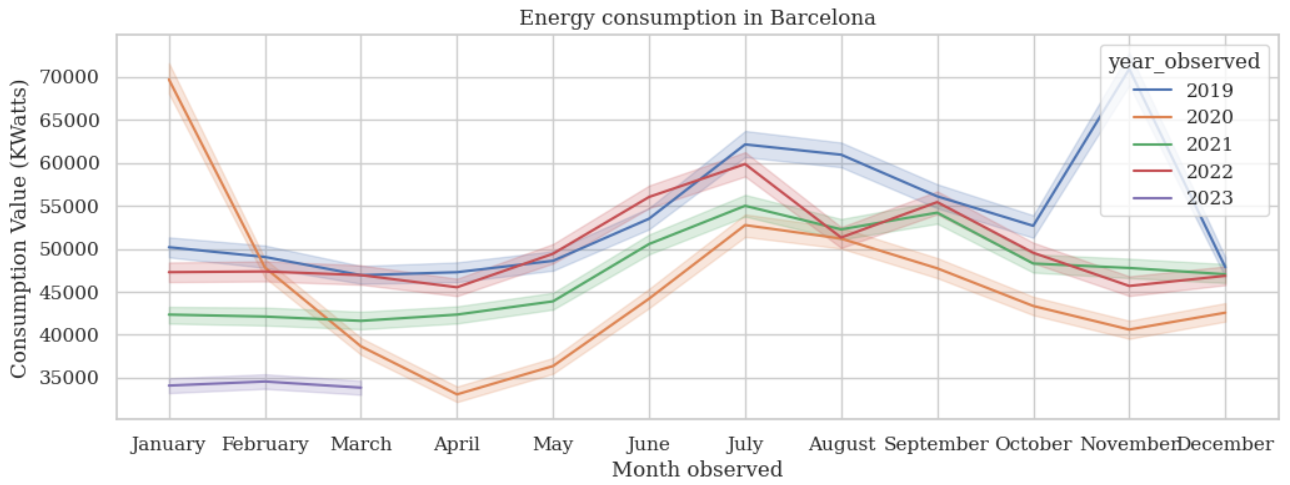
\includegraphics[width=13 cm]{imatges/energy_bcn_time_series.png}
\caption{\label{fig:energy_bcn_time_series} Time series of energy consumption in service buildings in Barcelona overlapped by year.}
\end{figure}

Due to computational performance issues, only the nighttime windows were used as it is when they should be idle, and an anomaly could be more feasibly detected. In figure~\ref{fig:energy_bcn_time_series} there is a distribution of the energy consumption in that time frame.

\begin{figure}[hbt]
\centering
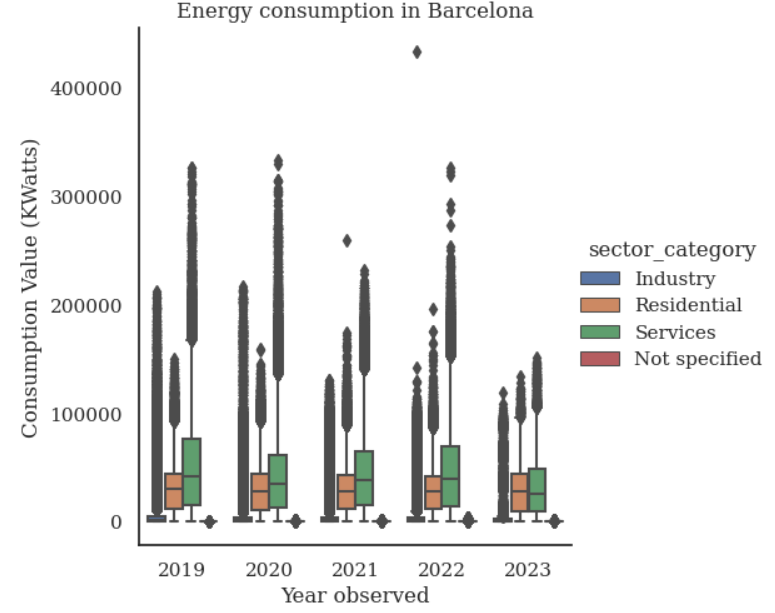
\includegraphics[width=13 cm]{imatges/energy_bcn_2019_2023-2.png}
\caption{\label{fig:energy_bcn_2019_2023} Distribution of energy consumption in Barcelona divided by economic field.}
\end{figure}

They have the accumulated data of 3 economic fields (industry, residential, and services, figure~\ref{fig:energy_bcn_2019_2023}). However, the scope of this project is to facilitate and assist the job at a governmental level, then the services buildings were selected to perform the modeling. 

To sum up the acquisition part, there were initially 1,051,455 records. As a result, performance was weak while using a mere 2GB of memory and limiting the choice to only one type of building. When focusing on public sector facilities, it is selected only to leave data on service buildings in the Gothic borough, leaving  327,180 records to work. This trial is restricted to the overnight period (from 18h to 5h) to lower the size of the dataset, as anomalies can be found when the service buildings should be consuming the least energy. We are now left with 130,872 records to perform ML techniques.

\renewcommand{\arraystretch}{1.5}
\begin{longtable}{ll}
\caption{Information of the dataset: \textit{Electricity consumption by postal code, economic sector, and time interval in the city of Barcelona} by ~\cite{ElectricityBCNOD}}  \\
\label{taula:InformationDataset}  \\
\textbf{Field}                & \textbf{Description}\\
\hline
\endfirsthead
\textbf{Field}                & \textbf{Description} \\
\hline
\endhead
%
Title                         & \parbox{7.5cm}{Electricity consumption by postal code, economic sector, and time interval in the city of Barcelona} \\
More information              & https://datadis.es  \\
Agenda 2030. SDG Principal    & SDG 7: Affordable and clean energy  \\
Agenda 2030. SDG Collateral 1 & N/A  \\
Agenda 2030. SDG Collateral 2 & N/A  \\
Source                        & \parbox{7.5cm}{Datadis. La plataforma de dades de consum elèctric} \\
Geolocation                   & No   \\
Long format available         & Yes  \\
Historical information        & Yes  \\
CKAN API available            & Yes  \\
Token required                & No \\
Management                    & Gerència Municipal \\
Department                    & \parbox{7.5cm}{Oficina Municipal de Dades - Departament d'Estadística i Difusió de Dades} \\
Publication Date              & 20/12/2022\\
Update frequency              & Monthly\\ 
\hline
\end{longtable}

\section{Data processing}

The dataset for \textit{electricity consumption in Barcelona} has a quite similar structure to the Swedish city's heat meter records of buildings used by~\cite{du2019clustering}. In this publication, they propose a data processing procedure (figure~\ref{fig:dataProcessing}) where they first pre-process the data, then detect the anomalies, extract some features, and then cluster the users' behavior, all based on heat consumption. 

\begin{figure}[hbt]
\centering
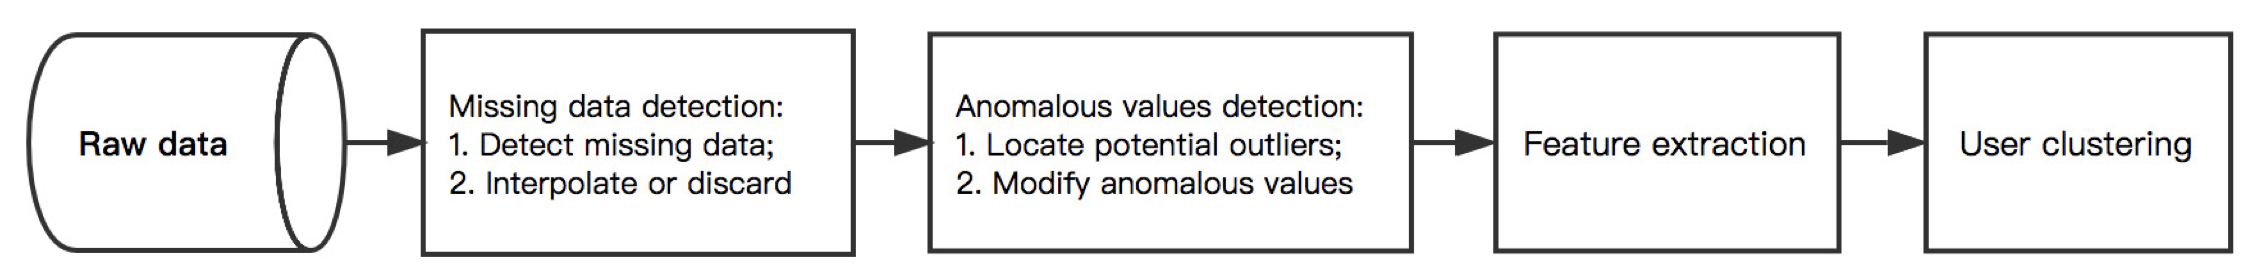
\includegraphics[width=13 cm]{imatges/dataProcessing.png}
\caption{\label{fig:dataProcessing} Data processing procedure proposed by~\cite{du2019clustering}.}
\end{figure}

\section{Data pre-processing}

To manage immense amounts of data, some of Apache Spark's built-in features from its library \textit{pyspark}, as mentioned by~\cite{liu2018scalable}, perform Data Analytics in Big Data. The structure to follow will be the one taken from Chapter~\ref{cap:estat}, Section~\ref{section:dataengineering} Data Engineering.

\subsection{Data cleaning}

The first step was to transform the data that was extracted with an incorrect data type. In this case, \textit{date\_observed}, \textit{year\_observed} and \textit{postal\_code}. Then it was time to translate the records as they were published in Catalan.

\subsection{Feature scaling}

In this part, the attributes were classified between categorical and numerical data. The former was normalized utilizing the MinMax method.

\subsection{Data integration}

From the \textit{date\_observed} new attributes were created to find the month and the day of the week the energy consumption tool place.

As mentioned in the review by ~\cite{moon2022toward}, calendars are an amazing tool to guide the difference between abnormal consumption and anomaly detection. It is for that reason that the Data on city festivals in Barcelona(table~\ref{taula:InformationFestivalsDataset}) was extracted and pre-processed following the same steps.

Only data was available from 2019 until 2022, which is perfect as that is the range necessary to train the data. Most holidays are periodic, on the same day, like Catalonia's National Day, on September 11th, or The Three Kings Parade on January 5th. A limitation is that the list does not take into account events such as concerts or football matches that move a massive amount of crowd, and that can have an effect on energy consumption and could cause a false anomaly. 

\begin{longtable}{ll}
\caption{Information of the dataset: \textit{Data on city festivals in the city of Barcelona} by~\cite{FestivalsBCNOD}}  \\
\label{taula:InformationFestivalsDataset}  \\
\hline
\textbf{Field}  & \textbf{Description} \\
\hline
\endfirsthead
\hline
\textbf{Field}  & \textbf{Description} \\
\hline
\endhead
%
Title  & \parbox{7cm}{Data on city festivals in the city of Barcelona}  \\
More information  & \parbox{7cm}{http://barcelonadadescultura.bcn.cat/ festes/dades?lang=en} \\
Agenda 2030. SDG Principal        & SDG 10: Reduced inequalities    \\
Agenda 2030. SDG Collateral 1     & SDG 11: Sustainable cities and communities   \\
Agenda 2030. SDG Collateral 2     & N/A  \\
Source                            & \parbox{7.5cm}{Secretaria Tècnica. Institut de Cultura. Ajuntament de Barcelona}\\
Geolocation                       & No  \\
Long format available             & Yes  \\
Historical information            & Yes  \\
CKAN API available                & Yes   \\
Token required                    & No    \\
Management                        & \parbox{7.5cm}{Gerència d'empresa, cultura i innovació} \\
Department & Pla de Sistemes  \\
Publication Date                  & 25/06/2014   \\
Update frequency                  & Annual   \\
\hline
\end{longtable}

\subsection{Feature Selection}

Once the two datasets, energy consumption and activities in the city, have been fused, the event location attribute and the postal code are compared to label if an event has occurred in that area. In this way, only this new feature is selected and the other two are discarded.

\subsection{Data discretization}

To classify if there has been an anomaly in the recorded data. The average of that day in previous years is calculated with a margin of 5\% above and below to determine the nature of  consumption.

After the selection of categorical features, these were treated to have a one-hot-encoding approach. In figure~\ref{fig:energy_bcn_heatmap} there are the relationships between the selected features after performing the discretization.

\begin{figure}[hbt]
\centering
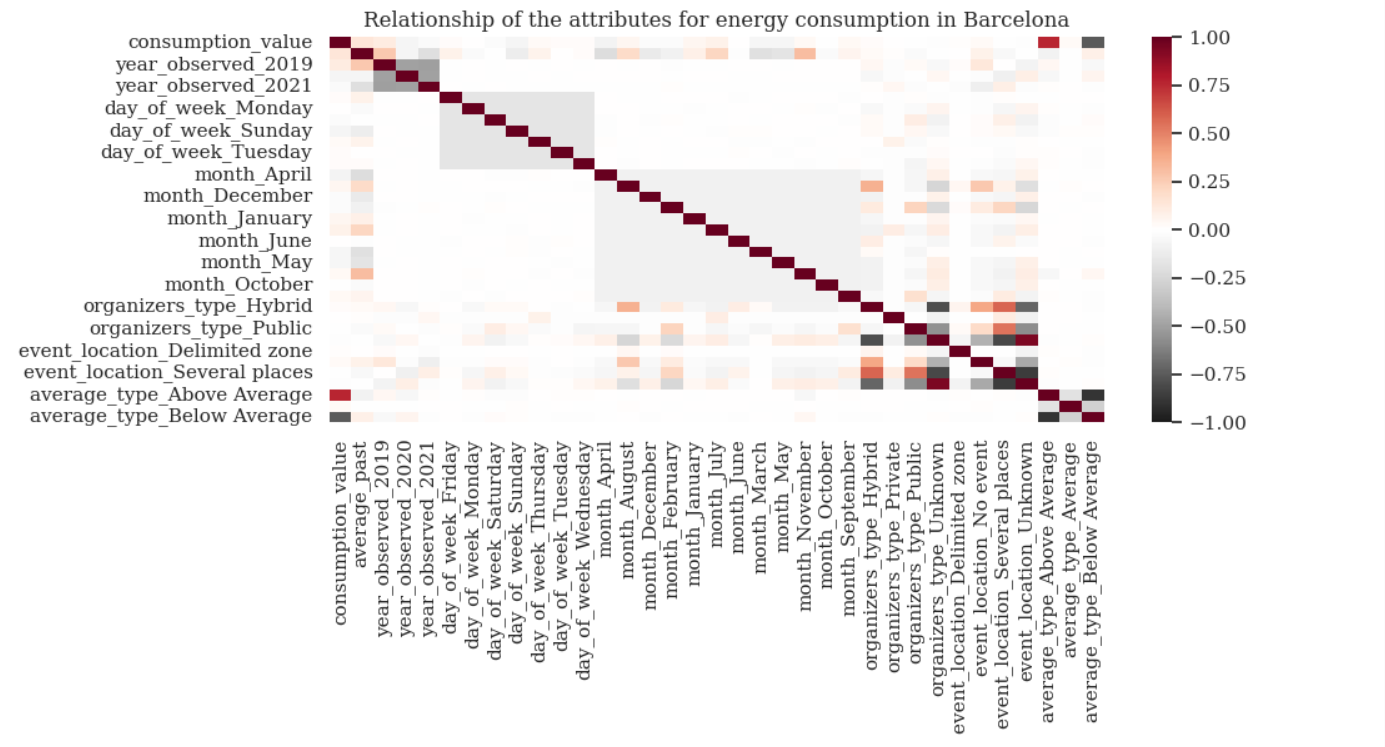
\includegraphics[width=13 cm]{imatges/energy_bcn_heatmap.png}
\caption{\label{fig:energy_bcn_heatmap} Features distribution and intensity in the electricity consumption dataset.}
\end{figure}

\section{Model building for Anomaly detection}

The purpose is to forecast the energy consumption and alert if the values are above or below the historic registers.
To do so, the data set was split into 2 groups. One to train the data from 2019 to 2022, and one to test and validate it as there is data in 2023.

The first part was to check if the time series was stationary. To assess it, the ADF (Augmented Dickey–Fuller) test was employed to determine if transformations should be made to the time series to stabilize it before further modeling or forecasting.

The hypotheses for this test are:

- H0: The time series has a unit root and is therefore non-stationary.

- H1: The time series does NOT have a unit root and is therefore stationary.

Once the time series is forecasted, then the classification and clustering will be performed to detect anomalies and find the pattern of energy consumption respectively.

\chapter{Results}
\label{cap:result}

\section{Forecasting the energy consumption}

The p-value (0.001) is smaller than 0.05. Consequently, there is sufficient statistical evidence to reject the null hypothesis and determine that we are facing a stationary time series.

ADF statistic: -3.9789548077150867

p-value: 0.0015248090038454789

Lags used: 22

Critical values: {'1\%': -3.4349056408696814, '5\%': -2.863552005375758, '10\%': -2.5678411776130114}

When performing the SAX + SARIMA approach proposed by~\cite{Carbone2017heating} ~\cite{fonseca2017unsupervised}. A \textit{UserWarning} was flagged, as there were not enough data points for identifying the seasonal ARMA's initial parameters, and except for variances they were set to zeros.

In view of this, a regression approach was considered that was used in data from smart energy meters to gain knowledge about households connected to the district heating network in Denmark~\cite{leiria2021using}.
  
The forecast was modeled to predict the energy consumption in the Gothic borough from March 2022 until March 2023. In figure~\ref{fig:energy_bcn_8002_forecasted} there are the results overlap with the recorded data in~\cite{ElectricityBCNOD}.

\begin{figure}[hbt]
\centering
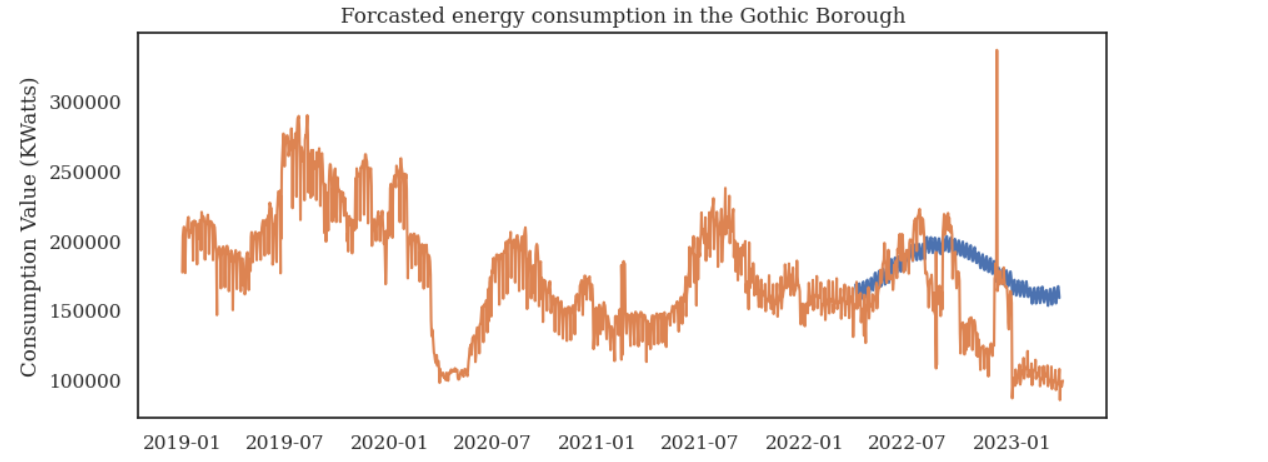
\includegraphics[width=13 cm]{imatges/energy_bcn_8002_forecasted.png}
\caption{\label{fig:energy_bcn_8002_forecasted} Time series of the original data set and the predicted energy consumption.}
\end{figure}

\section{Anomaly detection}

To classify if there has been an anomaly in the forecasted data. Using the previous consumption calculated in the data discretization with the above and below margin of 5\%. With that feature that determines if the recorded data is within the average or not, the training and validation data sets were divided. The first one had the data from January 1st, 2019, until December 31st, 2022, and the second one had the 2023 data.

The approaches followed from the energy field of study were: 

- KNN by~\cite{himeur2020data}

- RF by~\cite{cerquitelli2017predicting}

However, approaches like the XGBoost(used by~\cite{Wang2021CAN},~\cite{karanfilovska2022analysis},~\cite{saheed2022machine}), and SVM (used by~\cite{Wang2017Taxis},~\cite{Nugraha2021rail } ) were also considered.

\subsection{Model evaluation}

As a result of so many record reductions due to computational resources, when testing the training set, the accuracy showed an overfitted outcome from KFold Cross-Validation:

- KNN: 99.45\%

- SVM → linear: 100.0\%

- SVM → Radial Basis Function: 100.0\%

In spite of this, the models on the forecasted data were conclusive. In table~\ref{taula:ModelEvaluation} the models have a similar accuracy. Nonetheless, the KNN model was more accurate and had fewer mislabeled points than the others. Still, there is a lot of room for improvement as the predictions are labeled as \textit{Average} non-average records (figure~\ref{fig:confusion_knn}) which could be harmful.

\begin{longtable}{lcc}
\caption{Model comparison for classification energy consumption}  \\
\label{taula:ModelEvaluation}  \\
\hline
\textbf{ML Model} & \textbf{Accuracy} & \textbf{Mislabeled points} \\ 
\hline
\endfirsthead
%
\endhead
%
KNN  & 88.09\%  & 10 out of 84  \\ \hline
RF    & 85.71\% & 12 out of 84 \\ \hline
SVM   & 85.71\%  & 12 out of 84  \\ \hline
XGBoost  & 85.71\%  & 12 out of 84  \\ \hline
\end{longtable}

\begin{figure}[hbt]
\centering
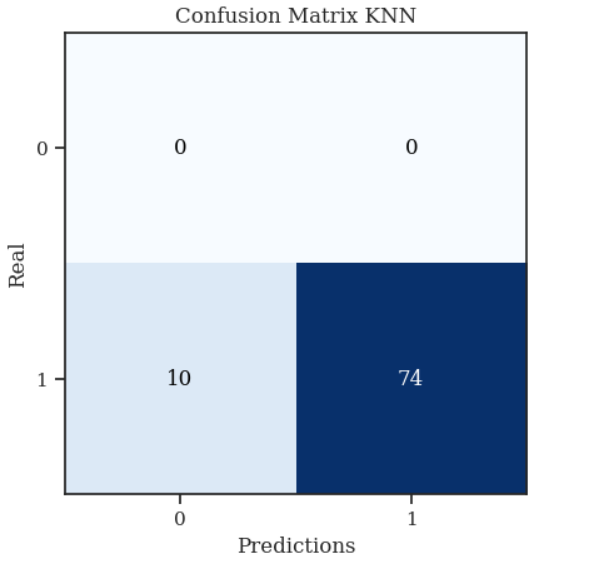
\includegraphics[width=7 cm]{imatges/confusion_knn.png}
\caption{\label{fig:confusion_knn} Confusion matrix according to the most accurate model trained.}
\end{figure}

To have an idea of what the other models were taking into account for the classification, in figure~\ref{fig:feature_importance_xgboost} is the importance of the trained features. 

In this case, the most important ones are the average type (below, above and average) and the consumption value despite having more attributes like the month or the activities that were happening that day.

\begin{figure}[hbt]
\centering
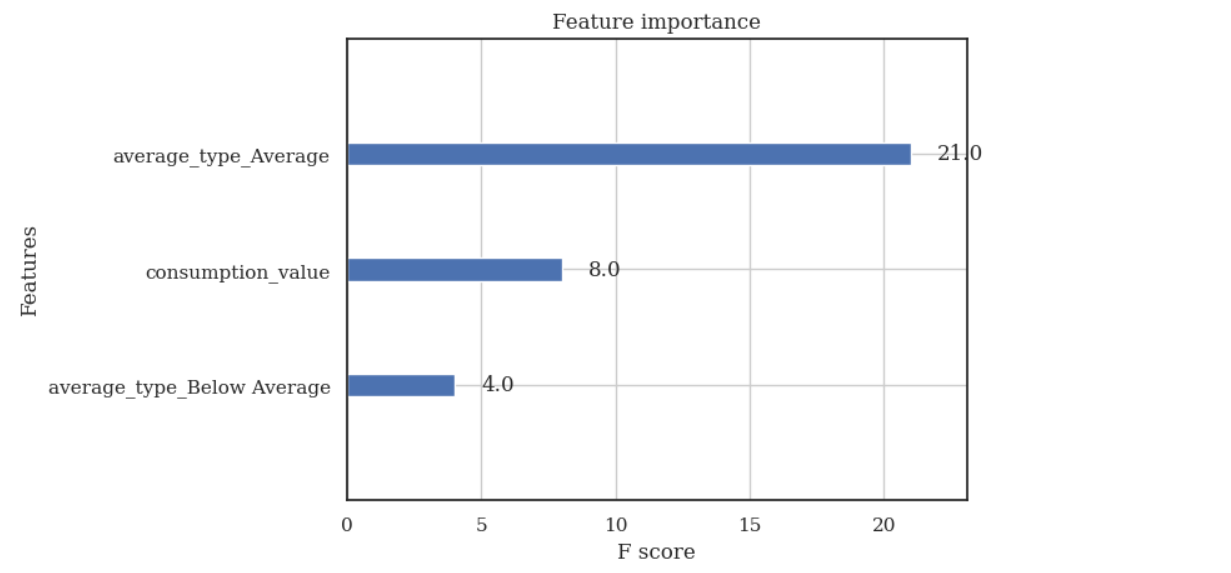
\includegraphics[width=13 cm]{imatges/feature_importance_xgboost.png}
\caption{\label{fig:feature_importance_xgboost} Feature importance in XGBoost model.}
\end{figure}

\section{Pattern consumption}

Unsupervised ML is when the algorithm just searches for patterns in the data, therefore, there is no outcome that can be predicted. In the K-Means case, the algorithm estimates the centroid of each set after randomly assigning each observation to a group. Then, in each iteration, it reassigns the data points to the nearest cluster's centroid.

Even though, in figure~\ref{f:Elbow} there is a turning like an elbow between k=2 and k=3.  For this dataset, the optimal number of clusters is 2 with a prediction strength of 1.0 (figure~\ref{f:kmeans_k2}).

\begin{figure}
 \centering
  \subfloat[Elbow Method]{
   \label{f:Elbow}
    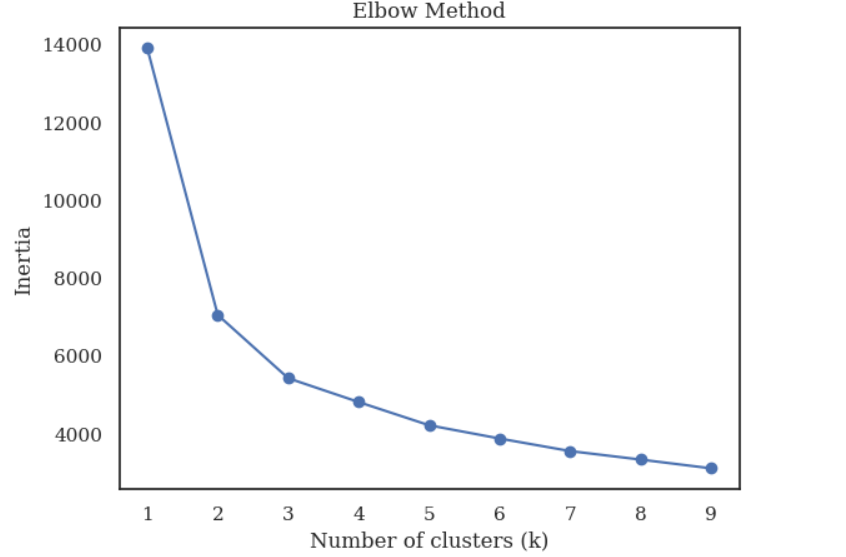
\includegraphics[width=0.5\textwidth]{imatges/elbow_kmeans.png}}
  \subfloat[K-Means with 2 clusters]{
   \label{f:kmeans_k2}
    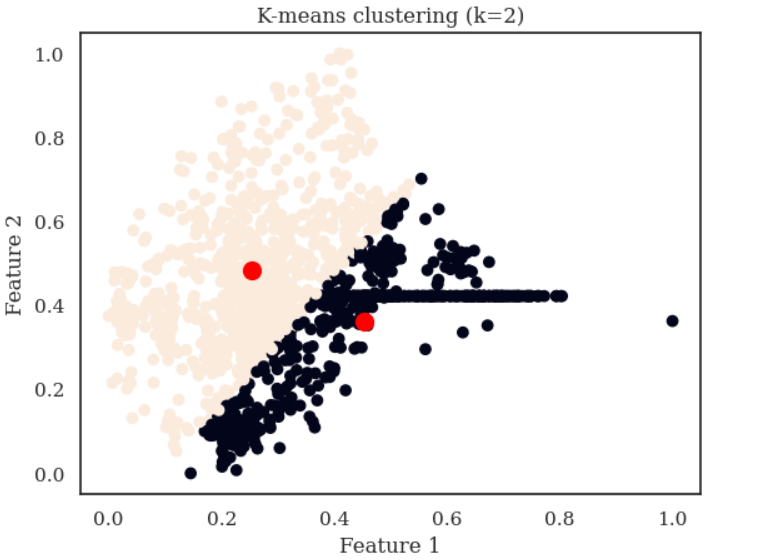
\includegraphics[width=0.45\textwidth]{imatges/kmeans_k2.png}}
 \caption{K-Means results}
 \label{f:KMeansresults}
\end{figure}

\begin{figure}[hbt]
\centering
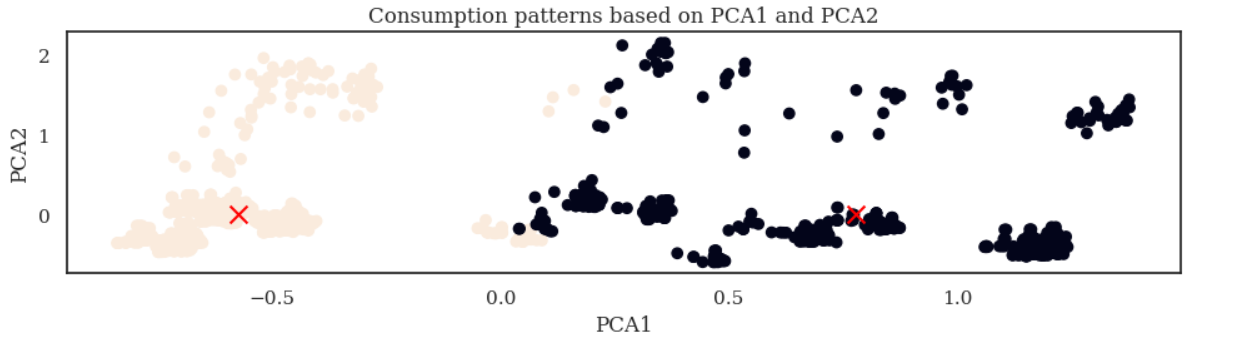
\includegraphics[width=13 cm]{imatges/patterns_pca_kmeans.png}
\caption{\label{fig:patterns_pca_kmeans} Clustering on the PCA components.}
\end{figure}

The dataset was minimize from 37 features to 2 features using principal component analysis (PCA). In figure~\ref{fig:patterns_pca_kmeans}, there is a representation of the clusters differentiated by a color parameter from the model's labels; and in figure~\ref{fig:effect_pca_kmeans}, there is the components' relationship with the training features for energy consumption.

\begin{figure}[hbt]
\centering
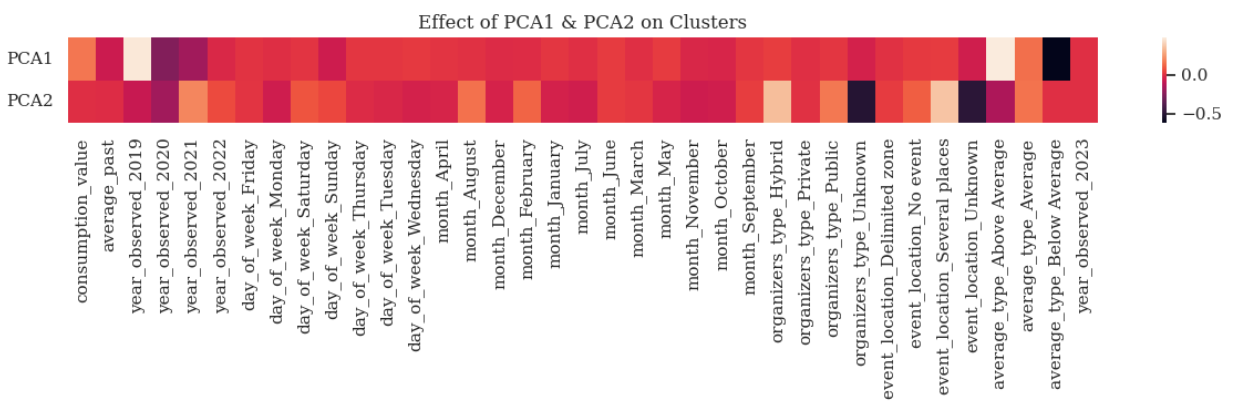
\includegraphics[width=13 cm]{imatges/effect_pca_kmeans.png}
\caption{\label{fig:effect_pca_kmeans} PCA on features.}
\end{figure}

\section{Communication}

The final outcome of this project is to spread the word and make it easier for people in the academia and the industry to gain more knowledge of detecting anomalies in smart cities with predictive models. A way to visualize the results found is by presenting a deliverable.

To use the resources learned throughout the master's degree, an \textit{ObervableHQ} was created with systematic review that can be found in: \url{https://observablehq.com/@andreaudg/anomaly-detection-lit-rev} (figure~\ref{fig:ObservableHQ}).

\begin{figure}[hbt]
\centering
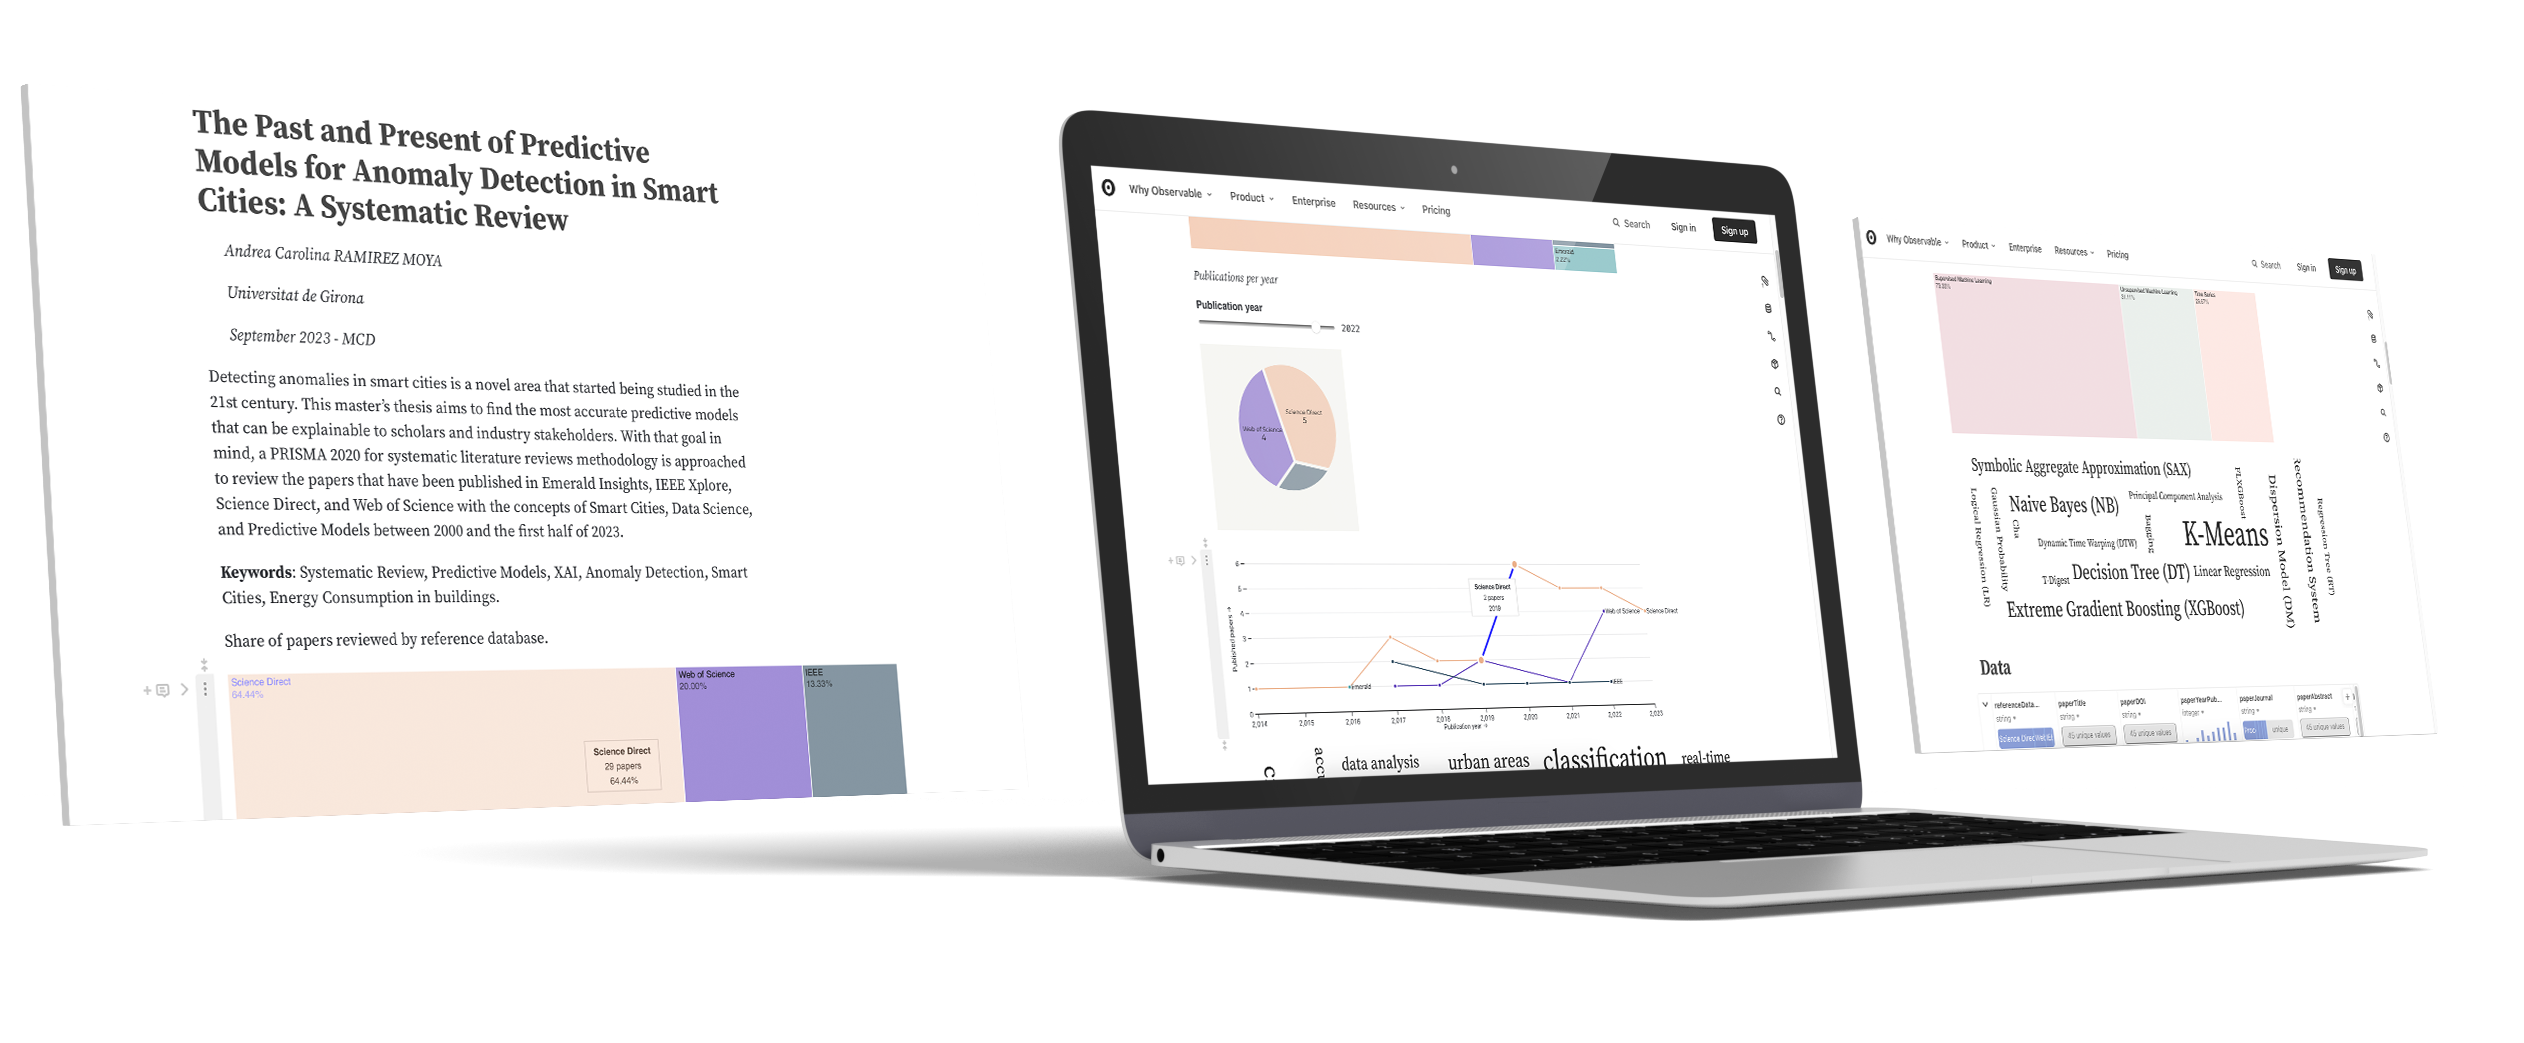
\includegraphics[width=13 cm]{imatges/observable_notebook.png}
\caption{\label{fig:ObservableHQ} Notebook in ObservableHQ.}
\end{figure}

Then to expose the experimentation results a dashboard was created to grasp the energy consumption in service buildings in the Gothic borough at night-time. It can be found in \url{https://lookerstudio.google.com/s/j_93RGA8KF0} (figure~\ref{fig:dashboard}).

\begin{figure}[hbt]
\centering
\includegraphics[width=15 cm]{imatges/dashboard_energy.png}
\caption{\label{fig:dashboard} Dashboard for energy consumption in service buildings in the Gothic borough at night-time.}
\end{figure}


\chapter{Conclusions and Future work}
\label{cap:concl}

To answer the initial research questions, 
\begin{itemize}
  \item \textit{Which area of a city has been studied the most, and which areas are in need of development?}
\end{itemize}
The city area studied the most is \textbf{transportation} which follows the trend within the scope of anomaly detection literature. It was closely followed by cybersecurity and energy. The areas that need development are the environment, people's mobility, and structures. There were no studies related to the living and security of the people.
\begin{itemize}
  \item \textit{Which predictive models are being used on anomaly detection in smart cities? Are those models using supervised or unsupervised ML techniques?}
\end{itemize}
The predictive models used the most to detect anomalies in smart cities are \textbf{classification}, which are \textbf{supervised ML techniques} such as RF, XGBoost, SVM, and KNN. However, some studies performed unsupervised clustering using K-Means and DBSCAN, depending on the anomaly type.
\begin{itemize}
  \item \textit{Which databases of bibliographical references has the most resources?}
\end{itemize}
The bibliographical reference database with the broader scope of published open access papers is \textbf{Science Direct}. \textit{IEEE} has a smaller section of conference papers instead of journals.

Despite referencing key ideas, several disqualified papers on the bibliographical reference databases did so because they correspond to a more theoretical than practical area. They emphasized more on potential solutions and upcoming difficulties. They discuss the possibilities in the area, notably the health sector and cybersecurity, but leave enormous room for future research. They have been used as case studies thus far, but there have yet to be any outcomes in anomaly detection. 

Throughout the development of the systematic literature review, I found limitations in the discussion of some topics, as they were mentioned in a latent way and just hinted at the subject. As a result, this opens an door for future research on data governance and the people's security in smart cities. In the future, the systematic review could be carried out using NLP (Natural Language Processing) tools to be able to address more publications. In this way, it would be more feasible to use search strategies that include more than 2.000 papers.

Papers are stuck in the analysis phase of the data collection and what happens after the models have predicted the anomalies is absent. They also do not present a data mining/acquisition approach; their smart data models are juxtaposed to data architecture, blending it into one topic.

The experimentation utilized 130.872 records, as there were initially more than one million records. For future work, more robust performance with more than 2GB of memory capacity is needed for the models to be trained in all the types of buildings in the city, in all boroughs, and at all times of the day, not only in the overnight period (from 18h to 5h), selected to lower the dataset size.

The operations part of ML and how these types of models can be brought to production can also be addressed.

\backmatter

\bibliographystyle{ThesisStyleBreakable}
\bibliography{biblio}

%\chapter{Appendix}
%\label{cap:appendix1}


%\printnomenclature

\end{document}
